% options:
% thesis=B bachelor's thesis
% thesis=M master's thesis
% czech thesis in Czech language
% slovak thesis in Slovak language
% english thesis in English language
% hidelinks remove colour boxes around hyperlinks

\documentclass[thesis=B,czech]{FITthesis}[2012/06/26]
\usepackage[utf8]{inputenc} % LaTeX source encoded as UTF-8
\usepackage{graphicx} %graphics files inclusion
% \usepackage{amsmath} %advanced maths
% \usepackage{amssymb} %additional math symbols
\usepackage{dirtree} %directory tree visualisation

% --------------------------------------------------------------------
% Default fixed font does not support bold face
\DeclareFixedFont{\ttb}{T1}{txtt}{bx}{n}{9} % for bold
\DeclareFixedFont{\ttm}{T1}{txtt}{m}{n}{9}  % for normal
% Custom colors
\usepackage{color}
\definecolor{deepblue}{rgb}{0,0,0.5}
\definecolor{deepred}{rgb}{0.6,0,0}
\definecolor{deepgreen}{rgb}{0,0.5,0}
\usepackage{listings}
\lstset{
     literate=%
         {á}{{\'a}}1
         {í}{{\'i}}1
         {é}{{\'e}}1
         {ý}{{\'y}}1
         {ú}{{\'u}}1
         {ó}{{\'o}}1
         {ě}{{\v{e}}}1
         {š}{{\v{s}}}1
         {č}{{\v{c}}}1
         {ř}{{\v{r}}}1
         {ž}{{\v{z}}}1
         {ď}{{\v{d}}}1
         {ť}{{\v{t}}}1
         {ň}{{\v{n}}}1                
         {ů}{{\r{u}}}1
         {Á}{{\'A}}1
         {Í}{{\'I}}1
         {É}{{\'E}}1
         {Ý}{{\'Y}}1
         {Ú}{{\'U}}1
         {Ó}{{\'O}}1
         {Ě}{{\v{E}}}1
         {Š}{{\v{S}}}1
         {Č}{{\v{C}}}1
         {Ř}{{\v{R}}}1
         {Ž}{{\v{Z}}}1
         {Ď}{{\v{D}}}1
         {Ť}{{\v{T}}}1
         {Ň}{{\v{N}}}1                
         {Ů}{{\r{U}}}1    
}
% Python style for highlighting
\newcommand\pythonstyle{\lstset{
language=Python,
basicstyle=\ttm,
otherkeywords={self},             % Add keywords here
keywordstyle=\ttb\color{deepblue},
emph={TestClubs,__init__,setUp,tearDown,testGet,testPost},          % Custom highlighting
emphstyle=\ttb\color{deepred},    % Custom highlighting style
stringstyle=\color{deepgreen},
% frame=tb,                         % Any extra options here
showstringspaces=false            % 
}}
% Python environment
\lstnewenvironment{python}[1][]
{
\pythonstyle
\lstset{#1}
}
{}
% Python for inline
\newcommand\pythoninline[1]{{\pythonstyle\lstinline!#1!}}
% --------------------------------------------------------------------
% JSON
\usepackage{xcolor}
\usepackage{listings}
\newcommand\JSONnumbervaluestyle{\color{blue}}
\newcommand\JSONstringvaluestyle{\color{red}}
% switch used as state variable
\newif\ifcolonfoundonthisline
\makeatletter
\lstdefinestyle{json}
{
  showstringspaces    = false,
  keywords            = {false,true},
  alsoletter          = 0123456789.,
  morestring          = [s]{"}{"},
  stringstyle         = \ifcolonfoundonthisline\JSONstringvaluestyle\fi,
  MoreSelectCharTable =%
    \lst@DefSaveDef{`:}\colon@json{\processColon@json},
  basicstyle          = \ttfamily,
  keywordstyle        = \ttfamily\bfseries,
}
% flip the switch if a colon is found in Pmode
\newcommand\processColon@json{%
  \colon@json%
  \ifnum\lst@mode=\lst@Pmode%
    \global\colonfoundonthislinetrue%
  \fi
}
\lst@AddToHook{Output}{%
  \ifcolonfoundonthisline%
    \ifnum\lst@mode=\lst@Pmode%
      \def\lst@thestyle{\JSONnumbervaluestyle}%
    \fi
  \fi
  %override by keyword style if a keyword is detected!
  \lsthk@DetectKeywords% 
}
% reset the switch at the end of line
\lst@AddToHook{EOL}%
  {\global\colonfoundonthislinefalse}
\makeatother
% --------------------------------------------------------------------

% % list of acronyms
% \usepackage[acronym,nonumberlist,toc,numberedsection=autolabel]{glossaries}
% \iflanguage{czech}{\renewcommand*{\acronymname}{Seznam pou{\v z}it{\' y}ch zkratek}}{}
% \makeglossaries

% % % % % % % % % % % % % % % % % % % % % % % % % % % % % % 
% ODTUD DAL VSE ZMENTE
% % % % % % % % % % % % % % % % % % % % % % % % % % % % % % 

\department{Katedra softwarového inženýrství}
\title{Systém pro skórování Ultimate~Frisbee~zápasů~-~backend}
\authorGN{Marek} %(křestní) jméno (jména) autora
\authorFN{Dostál} %příjmení autora
\authorWithDegrees{Marek Dostál} %jméno autora včetně současných akademických titulů
\supervisor{Ing. Jiří Hunka}
\acknowledgements{Doplňte, máte-li komu a za co děkovat. V~opačném případě úplně odstraňte tento příkaz.}
\abstractCS{
Tato bakalářská práce se zabývá návrhem a realizací backendu webové aplikace
sloužící ke správě turnajů a tvorbě statistik v Ultimate Frisbee.
Podstatou řešení je vývoj RESTového rozhraní v Pythonu a jeho nasazení do provozu pomocí uWSGI.
Výsledkem je fungující webová aplikace a~její backend nezávislý na~frontendu.  
}

\abstractEN{Sem doplňte ekvivalent abstraktu Vaší práce v~angličtině.}
\placeForDeclarationOfAuthenticity{V~Praze}
\declarationOfAuthenticityOption{4} %volba Prohlášení (číslo 1-6)
\keywordsCS{webová služba, REST API, Python, framework Falcon, Ultimate Frisbee}
\keywordsEN{Nahraďte seznamem klíčových slov v angličtině oddělených čárkou.}

\usepackage{fancyvrb}

\renewcommand{\arraystretch}{1.3}

\begin{document}
 
 % TODO: podivat se na to, co rikal Hunka + problemy pri implementaci
 
% \newacronym{CVUT}{{\v C}VUT}{{\v C}esk{\' e} vysok{\' e} u{\v c}en{\' i} technick{\' e} v Praze}
% \newacronym{FIT}{FIT}{Fakulta informa{\v c}n{\' i}ch technologi{\' i}}

\chapter{Úvod do problematiky}

\indent

V první kapitole bychom se měli seznámit s pojmem Ultimate Frisbee. Dále pak nastíníme
problematiku pořádání turnajů v tomto minoritním sportu.

\section{Co je to Ultimate Frisbee}

\indent

Ultimate Frisbee je mladý a dynamicky se rozvíjející sport s létajícím talířem,
který se hraje od roku 1968 \cite{cald-ultimate}. Hraje jej přibližně sedm miliónů
hráčů ve více než 80 zemích světa a jeho popularita rok od roku stoupá \cite{usa-ultimate}.
Během posledních několika let je například běžné sledovat živé přenosy na sportovním kanálu ESPN
z Amerických soutěží, především profesionální ligy AUDL. Ultimate v roce 2015 dokonce získalo
uznání od Mezinárodního olympijského výboru \cite{cald-uznani}. Nejčastěji se hraje v kategoriích
open (muži), ženy, mix (smíšené týmy mužů a žen), junioři (do 19 let) a masters (nad 33 let).

\subsection{Pravidla}

\indent

Popularitě přidává fakt, že jde o celkem vzato nenáročnou hru na vybavení s jednoduchými pravidly:

\begin{quote}
Ultimate je kolektivní bezkontaktní sport, v němž vítězí tým, který má na konci hrací doby
vyšší počet bodů. Hraje se na hřišti o rozměrech cca 100x37 metrů (délka fotbalového hřiště,
polovina jeho šířky). Na obou koncích hřiště jsou vyznačeny koncové zóny o hloubce cca 18 metrů.

V ultimate proti sobě hrají dva sedmičlenné týmy. Smyslem hry je pomocí přihrávek dopravit disk
do soupeřovy koncové zóny a jeho chycením v zóně získat bod. Po chycení disku se hráč musí
zastavit a do 10 vteřin disk přihrát spoluhráči. Povoleným pohybem hráče s diskem je pivotování,
tedy otáčení se kolem vlastní osy s jednou nohou pevně na zemi. V ultimate hráči často střídají
útok a obranu při ztrátě disku, ke které dochází záhozem disku do autu, na zem, jeho zachycením
soupeřem nebo při dlouhém držení disku. Není povolen fyzický kontakt mezi hráči ani přetahování
o disk (\cite{cald-ultimate}).
\end{quote}

\begin{figure}[ht!]
\centering
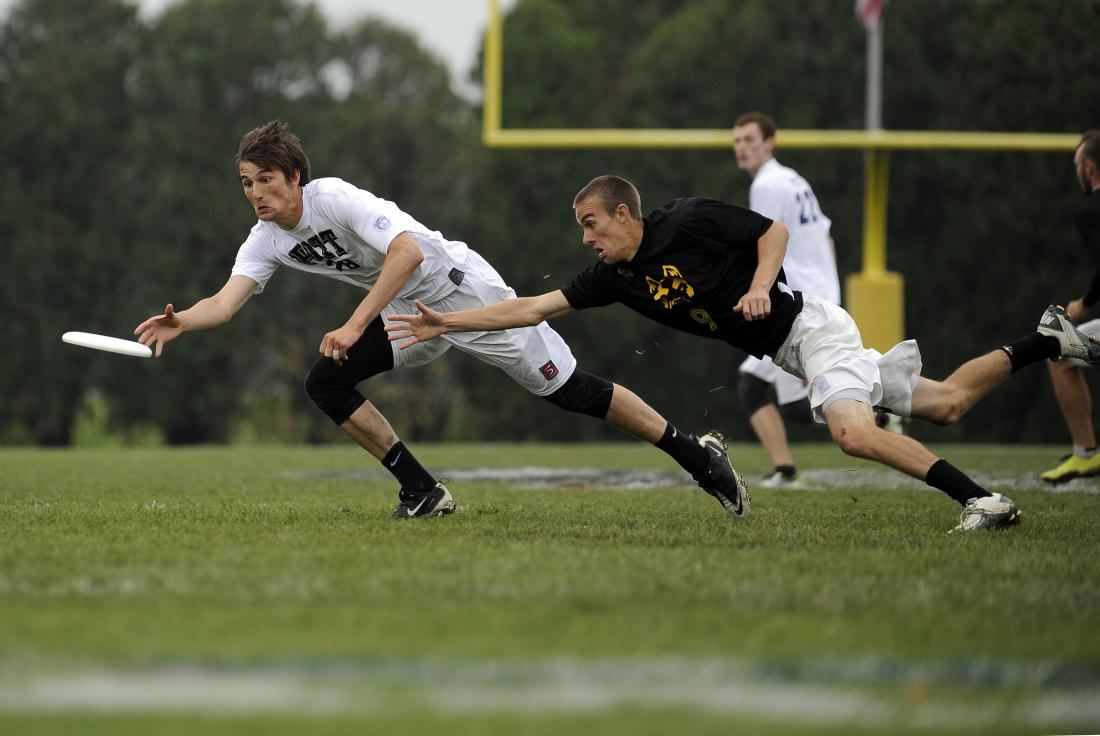
\includegraphics[width=130mm]{./images/ultimate-frisbee.jpg}
\caption{Fotografie z amerického časopisu TIME ze zápasu mezi univerzitními týmy z Pittsburgu a Floridy \cite{ultimate-time}\label{overflow}}
\end{figure}


\subsection{Spirit of the Game}

\indent

Už od počátku je Ultimate Frisbee založeno na sportovním duchu, který klade odpovědnost
za fair play na samotné hráče. Předpokládá se vysoce soutěživá hra, ne však za cenu ztráty
vzájemné ohleduplnosti a vytracení radosti ze hry. Všechny přetupky na hřišti i mimo něj jsou
řešeny samotnými hráči. Jako jediná sportovní hra se tak obejde bez rozhodčích, a to i
na nejvyšších soutěžích, kterými jsou mistrovství Evropy a světa.

\medskip

Hraní fairplay je otázka cti. Na každém turnaji je vyhlašována cena Spirit of the Game,
která je cenou pro ty, kteří se chovali nejčestněji. Po každém zápase se týmy navzájem ohodnotí
v podobě číselného hodnocení a cenu pak získá tým s nejvyšším průměrem. Cena Spirit of the Game
je ceněna obdobně jako 1. místo.

\subsection{Ultimate v České republice}

\indent

V České republice zastřešuje sporty s létajícím talířem již od roku 1991\cite{cald-historie} Česká asociace
lé\-ta\-jícícho disku (dále jen ``ČALD''). V celé republice eviduje desítky zaregistrovaných
klubů (často zvaných oddílů), které se mezi sebou utkávají v rámci celého roku na akcích zvané turnaje.
Jenom za loňský rok jich bylo na našem území přes třicet \cite{cald-kalendar}.

\medskip

Většina turnajů nebo mistrovství pak trvá zpravidla více dnů, během kterých se odehrají desítky
utkání. A s přibývajícím počtem hráčů a fanoušků vzniká čím dál větší poptávka po online
přenosech a statistikách z těchto akcí.

% TODO: Bude potreba doplnit, protoze se jedna o dulezity pojem, ktery bude pak zpracovan.

%\subsection{Jak probíhá typický turnaj - IDEA - nedokonceno}

%\indent

%Několik dní před turnajem se zveřejní rozpis, zpravidla v podobě dokumentu na Google Drive apod.
%Ten je pak během turnajem editovaný a slouží jako jediný zdroj výsledků, který ... 

%Nejdůležitejším údajem jsou výsledky z jednotlivých zápasů. Ty jsou nejčastěji zapisovány
%na papír, který je vystaven na viditelném místě, aby si jej mohlo prohlédnout co nejvíce lidí.

%\medskip

%Částečně tyto procesy nahrazuje mobilní aplikace Catcher, ke které se ještě dostaneme.

% Vsechno se doposud pise na papir a je to proste cely na prd.
% TODO: Kdo vsechno, kolik lidi, na turnaji pobyva. Kolik probiha zapasu, treba i paralelne, kdo se o nej stara (navrh ma mobilni app). Co vsechno se da vycist z vysledku.
% TODO: Jeste doplnit dal.

% TODO: sem prijde rest api

\chapter{Úvod do problematiky}

\indent

V první kapitole bychom se měli seznámit s pojmem Ultimate Frisbee. Dále pak nastíníme
problematiku pořádání turnajů v tomto minoritním sportu.

\section{Co je to Ultimate Frisbee}

\indent

Ultimate Frisbee je mladý a dynamicky se rozvíjející sport s létajícím talířem,
který se hraje od roku 1968 \cite{cald-ultimate}. Hraje jej přibližně sedm miliónů
hráčů ve více než 80 zemích světa a jeho popularita rok od roku stoupá \cite{usa-ultimate}.
Během posledních několika let je například běžné sledovat živé přenosy na sportovním kanálu ESPN
z Amerických soutěží, především profesionální ligy AUDL. Ultimate v roce 2015 dokonce získalo
uznání od Mezinárodního olympijského výboru \cite{cald-uznani}. Nejčastěji se hraje v kategoriích
open (muži), ženy, mix (smíšené týmy mužů a žen), junioři (do 19 let) a masters (nad 33 let).

\subsection{Pravidla}

\indent

Popularitě přidává fakt, že jde o celkem vzato nenáročnou hru na vybavení s jednoduchými pravidly:

\begin{quote}
Ultimate je kolektivní bezkontaktní sport, v němž vítězí tým, který má na konci hrací doby
vyšší počet bodů. Hraje se na hřišti o rozměrech cca 100x37 metrů (délka fotbalového hřiště,
polovina jeho šířky). Na obou koncích hřiště jsou vyznačeny koncové zóny o hloubce cca 18 metrů.

V ultimate proti sobě hrají dva sedmičlenné týmy. Smyslem hry je pomocí přihrávek dopravit disk
do soupeřovy koncové zóny a jeho chycením v zóně získat bod. Po chycení disku se hráč musí
zastavit a do 10 vteřin disk přihrát spoluhráči. Povoleným pohybem hráče s diskem je pivotování,
tedy otáčení se kolem vlastní osy s jednou nohou pevně na zemi. V ultimate hráči často střídají
útok a obranu při ztrátě disku, ke které dochází záhozem disku do autu, na zem, jeho zachycením
soupeřem nebo při dlouhém držení disku. Není povolen fyzický kontakt mezi hráči ani přetahování
o disk (\cite{cald-ultimate}).
\end{quote}

\begin{figure}[ht!]
\centering
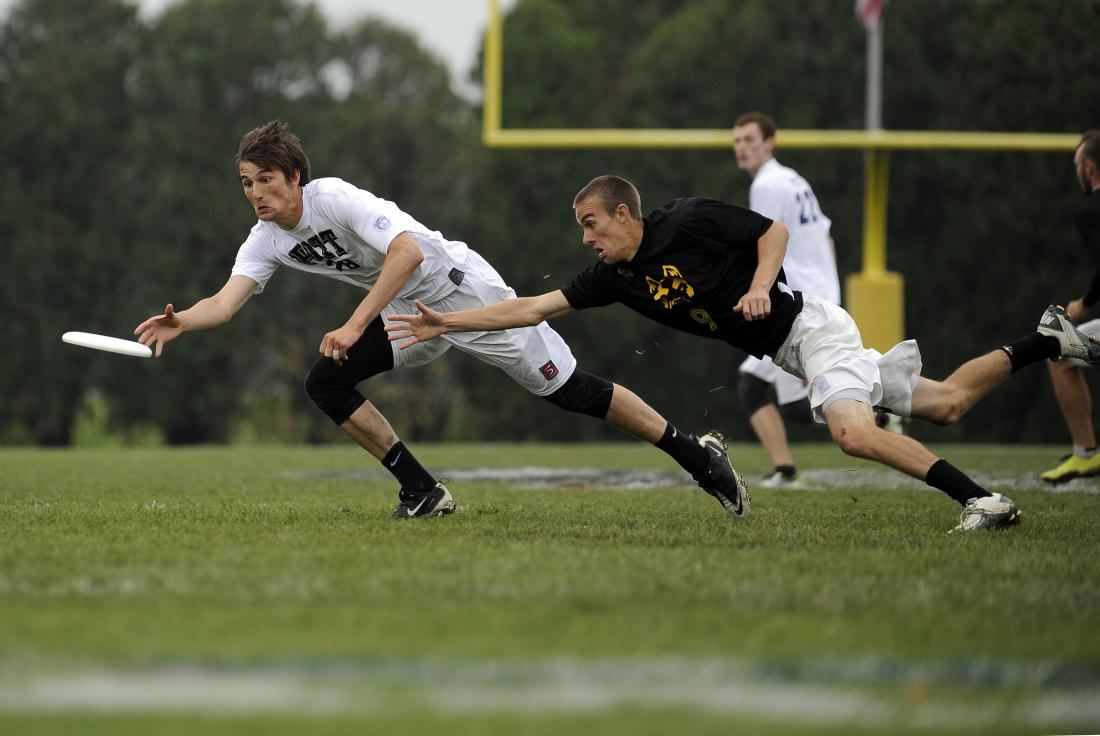
\includegraphics[width=130mm]{./images/ultimate-frisbee.jpg}
\caption{Fotografie z amerického časopisu TIME ze zápasu mezi univerzitními týmy z Pittsburgu a Floridy \cite{ultimate-time}\label{overflow}}
\end{figure}


\subsection{Spirit of the Game}

\indent

Už od počátku je Ultimate Frisbee založeno na sportovním duchu, který klade odpovědnost
za fair play na samotné hráče. Předpokládá se vysoce soutěživá hra, ne však za cenu ztráty
vzájemné ohleduplnosti a vytracení radosti ze hry. Všechny přetupky na hřišti i mimo něj jsou
řešeny samotnými hráči. Jako jediná sportovní hra se tak obejde bez rozhodčích, a to i
na nejvyšších soutěžích, kterými jsou mistrovství Evropy a světa.

\medskip

Hraní fairplay je otázka cti. Na každém turnaji je vyhlašována cena Spirit of the Game,
která je cenou pro ty, kteří se chovali nejčestněji. Po každém zápase se týmy navzájem ohodnotí
v podobě číselného hodnocení a cenu pak získá tým s nejvyšším průměrem. Cena Spirit of the Game
je ceněna obdobně jako 1. místo.

\subsection{Ultimate v České republice}

\indent

V České republice zastřešuje sporty s létajícím talířem již od roku 1991\cite{cald-historie} Česká asociace
lé\-ta\-jícícho disku (dále jen ``ČALD''). V celé republice eviduje desítky zaregistrovaných
klubů (často zvaných oddílů), které se mezi sebou utkávají v rámci celého roku na akcích zvané turnaje.
Jenom za loňský rok jich bylo na našem území přes třicet \cite{cald-kalendar}.

\medskip

Většina turnajů nebo mistrovství pak trvá zpravidla více dnů, během kterých se odehrají desítky
utkání. A s přibývajícím počtem hráčů a fanoušků vzniká čím dál větší poptávka po online
přenosech a statistikách z těchto akcí.

% TODO: Bude potreba doplnit, protoze se jedna o dulezity pojem, ktery bude pak zpracovan.

%\subsection{Jak probíhá typický turnaj - IDEA - nedokonceno}

%\indent

%Několik dní před turnajem se zveřejní rozpis, zpravidla v podobě dokumentu na Google Drive apod.
%Ten je pak během turnajem editovaný a slouží jako jediný zdroj výsledků, který ... 

%Nejdůležitejším údajem jsou výsledky z jednotlivých zápasů. Ty jsou nejčastěji zapisovány
%na papír, který je vystaven na viditelném místě, aby si jej mohlo prohlédnout co nejvíce lidí.

%\medskip

%Částečně tyto procesy nahrazuje mobilní aplikace Catcher, ke které se ještě dostaneme.

% Vsechno se doposud pise na papir a je to proste cely na prd.
% TODO: Kdo vsechno, kolik lidi, na turnaji pobyva. Kolik probiha zapasu, treba i paralelne, kdo se o nej stara (navrh ma mobilni app). Co vsechno se da vycist z vysledku.
% TODO: Jeste doplnit dal.

% TODO: sem prijde rest api
 
\chapter{Specifikace požadavků}

Zadání této práce vzniklo původně z požadavku na rozšíření již fungující mobilní aplikace Catcher.
Její autor mne na konci roku 2015 oslovil s nápadem vylepšit její serverou část a doplnit API,
které by mohla využívat libovolná klientská aplikace. Po rychlé analýze jsme však oba došli k závěru,
že bude lepší navrhnout nový backend, protože ten starý nebyl reálně vůbec rozšiřitelný. %Jméno projektu je pojmenované po...

Finálním řešením je tak webová služba, která poskytuje kompletní rozhraní,
tzn. že jde o zcela nezávislou vrstvu mezi frontendem a backendem.
Protože výsledek mé práce má později nahradit nevyhovující backend staré aplikace, ponechal jsem celému projektu jméno Catcher.

\section{Požadavky na Catchera}

Protože se v komunitě hráčů i organizátorů turnajů jako aktivní hráč sám pohybuji,
nebyl problém stanovit funkční i nefunkční požadavky na vznikající službu.

\subsection{Funkční požadavky}

\begin{description}
  \item[Import a export dat]
    Systém umožňuje import oddílů a jeho hráčů z databáze ČALD.
  \item[Rozpis zápasů]
    Oprávněná role může vytvořit svůj vlastní turnaj a vložit seznam všech zápasů,
    které se budou hrát. Vytvořený rozpis zápasů systém již doplňuje automaticky na základě
    odehraných výsledků (např.~vítěze semifinále automaticky posune do finále). Ve chvíli,
    kdy to bude již možné, doplní celkové pořadí turnaje. Automatické doplnění se
    týká i~souhrnné tabulky vzájemných hodnocení v kategorii SOTG.
  \item[Zadávání dat v rámci turnaje]
    Každý tým má možnost vytvořit vlastní soupisku na turnaj. Systém pak umožňuje
    v průběhu turnaje zadávat konkrétní údaje:
    \begin{itemize}
      \item průběžné skóre zápasů nebo jejich závěrečný výsledek
      \item skórující a asistující hráč
      \item hodnocení SOTG
    \end{itemize}
  \item[Tvorba statistik]
    Systém tvoří detailní statistiky hráčů, týmů a zápasů (obdržené a udělené body,
    počet asistencí, průměrná hodnota SOTG).
\end{description}

\subsection{Nefunkční požadavky}

\begin{description}
  \item[Snadná rozšířitelnost]
    Už nyní evidujeme změny, o~které je zájem, ale nejsou předmětem této práce.
    I proto je nutné projekt dokončit tak, aby byl v~budoucnu snadno rozšiřitelný nebo
    modifikovatelný.
  \item[Nízká cena]
    Cílem není vytvořit výdělečný projekt, ale fungující službu pro~několik stovek hráčů
    a~fanoušků v~České republice. I~proto je požadavkem použití volně dostupných
    knihoven a~technologií.
  \item[Výkon]
    Podle celkem jednoduchých odhadů lze usoudit, že aplikaci budou čekat výkyvy v provozu.
    Většina zápisů a čtění dat probíhá během samotných turnajů. Během špičky nebude počet požadavků za sekundu
    větší než několik desítek. I proto není na celkový výkon kladen žádný zvláštní požadavek.
    Systém by každopádně měl minimálně 95 \% žádostí zpracovat do jedné sekundy.
  \item[Spolehlivost]
    Spolehlivost je základem pro funkční běh Catchera. Velká část operací, včetně chybných budou
    zapisovány do souborů pro snadné odhalení chyb. Obnova musí být proveditelná ze zálohovacích souborů.
    %V případě výpadku by měl být informován administrátor pomocí SMS nebo e-mailu.
    \item[Bezpečnost]
    Systém musí jednoznačně určit a ověřit uživatele, který přistupuje k rozhraní Catchera. Zároveň
    musí existovat možnost za chodu přidávat, odebírat nebo měnit oprávnění uživatelů.
    % Dále pak systém musí být datově integritní, tzn. že obsah zpráv nebude při přenosu změněn.
    Pro tento projekt není nutné používat HTTPS\footnote{Hypertext Transfer Protocol Secure} protokol.
  \item[Nároky na hardware]
    Systém musí být schopen běžet na běžných serverech s ne více jak 1024 MB RAM\footnote{Random Access Memory}.
  \item[Formát importu]
    Pro import soupisek musí systém umět číst data ve formátu, který ČALD pro export používá.
  \item[Vytvoření dokumentace]
    Pro vývoj klientských aplikací je potřeba vytvořit dostatečně detailní dokumentaci rozhraní.
\end{description}

\section{Uživatelské role}

\begin{description}
  \item[Nepřihlášený návštěvník]
    Jde o nejčastější přístup k aplikaci. Slouží k zobrazení všech statistik (aktuální skóre,
    statistika všech hráčů, hodnocení SOTG). Nemůže žádná data vytvářet nebo modifikovat
    a nevyžaduje přihlášení.
  \item[Organizátor]
    Účet pod touto rolí může vytvořit kdokoliv pouhou registrací. Po příhlášení lze přídávat
    nové turnaje a ty následně spravovat. Tím se rozumí tvorba rozpisu zápasů a seznamu účastníků.
    Dále může zadávat průběžné a výsledné skóre zápasů, skórující a asistující hráče a vidí
    na~tabulku vzájemných hodnocení SOTG pro~účely vyhlášení vítěze.
    Tato tabulka je pro ostatní role až do~ukončení turnaje nezobrazitelná.
  \item[Klubový/oddílový účet]
    Pro účely odevzdávání hodnocení SOTG a úprav v týmové soupisce je vytvořen pro každý oddíl
    jeden společný účet. Tento účet má možnost vytvořit pouze administrátor. Přihlašovací údaje pak
    získá zástupce klubu a je pouze na něm, kdo z jeho oddílu bude spravovat vytvořený učet.
    Součástí klubu může být více týmů, např. mužský a~ženský tým nebo A-tým a B-tým.
  \item[Administrátor]
    Má plnou kontrolu nad správou účtů a nad daty v databázi.
    Jeho možnosti vznikají sjednocením všech ostatních rolí.
\end{description}

\section{Případy užití}
\label{sec:use_case}

Následující část popisuje nejběžnější případy užití. V návrhu rozhraní jde
o~jednu z~nejdůležitejších součastí, protože určuje směr návrhu. Výsledné API by tak mělo
pokrývat všechny níže uvedené případy. Seznam zachycuje jednotlivé požadavky
a~jejich popis:

\subsection*{Import}
  \begin{description}
    \item[UC1: Import dat z databáze ČALD]
      Doplňuje seznam oddílů a jejich hrá\-čů do databáze Catchera. Manuálně lze stáhnout
      aktuální data z ČALD databáze a doplnit doposud aktuální data v databázi.
  \end{description}

\subsection*{Uživatelé}
  \begin{description}
    \item[UC2: Registruje nového uživatele]
      Kdokoliv se může stát registrovaným uživatelem s rolí organizátor. Stačí se zaregistrovat s platným e-mailem.
      Klubové účty vytváří administrátor.
    \item[UC3: Autentizuje uživatele]
      Určí skutečnou identitu uživatele. Jinými slo\-vy jej přihlásí. Po úspěšném přihlášení je uživateli vrácen
      přístupový token pro vykonávaní dalších požadavků (více k sekci~\ref{sec:security}).
    \item[UC4: Odesílá zapomenuté heslo]
      Při ztrátě hesla lze požádat o odeslání nového náhodně vygenerovaného na e-mail, který uživatel zadal při své registraci.
  \end{description}

\subsection*{Oddíly}
  \begin{description}
    \item[UC5: Vytvoří oddíl]
      Uloží nový oddíl do databáze. Ukládá se u~něj jméno, město a~země původu.
    \item[UC6: Získá oddíly]
      Vrátí informace o jednom nebo více oddílech.
    \item[UC7: Edituje oddíl]
      Upraví informace o oddílu.
    \item[UC8: Smaže oddíl]
      Smaže oddíl z databáze.
  \end{description}

\subsection*{Hráči}
  \begin{description}
    \item[UC9: Vytvoří hráče]
      Vytvoří nového hráče, u kterého lze vytvořit vazba pouze k jednomu oddílu.
      Kromě jména a příjmení u něj lze uložit číslo dresu a jeho přezdívku.
    \item[UC10: Získá hráče]
      Vrátí informace o jednom nebo více hráčích.
    \item[UC11: Edituje hráče]
      Upraví informace o hráči.
    \item[UC12: Smaže hráče]
      Smaže hráče z databáze.
  \end{description}

\subsection*{Týmy}
  \begin{description}
    \item[UC13: Vytvoří tým]
      Vytvoří tým spadající pod konkrétní oddíl. Týmu se musí přiřadit stupeň a divize (např. A-tým ženy).
    \item[UC14: Získá týmy]
      Vrátí informace o jednom nebo více týmech.
    \item[UC15: Edituje tým]
      Upraví informace o týmu.
    \item[UC16: Smaže tým]
      Smaže tým z databáze.
  \end{description}

\subsection*{Turnaje}
  \begin{description}
    \item[UC17: Vytvoří turnaj]
      Uloží nový turnaj včetně účastníků turnaje, základních skupin a zápasů ve skupinách a play-off.
    \item[UC18: Edituje turnaj]
      Upraví informace o turnaji nebo změní jeho stav.
    \item[UC19: Získá turnaje]
      Vrátí informace o jednom nebo více turnajích.
    \item[UC20: Získá konečné pořadí]
      Získá známé pořadí týmů na turnaji a pokud turnaj již skončil, zobrazí i hodnocení SOTG.
  \end{description}

\subsubsection*{Týmové soupisky}
  \begin{description}
    \item[UC21: Připsat hráče na soupisku]
      Týmům na turnaji lze přiřadit hráče, tzn. vytvořit týmové soupisky. Hráčům ze soupisky
      pak lze připisovat body na turnaji. Každý hráč může hrát na turnaji pouze za jeden tým.
    \item[UC22: Získá soupisky]
      Vrátí soupisku konkrétního týmu nebo seznam hráčů napříč celým turnajem. Včetně jejich statistik a seřazení dle úspěšnosti.
    \item[UC23: Odebere hráče ze soupisky]
      Jestliže hráč nedisponuje žádnými statistikami a nestihl ještě do žádného zápasu zasáhnout, je možné jej odstranit ze soupisky.
  \end{description}

\subsubsection*{Skupiny a zápasy}
  \begin{description}
    \item[UC24: Získá skupiny]
      Vrátí informace o vybraných skupinách. Seznam týmů včetně jejich vzájemného skóre a pořadí ve skupině.
    \item[UC25: Získá zápasy]
      Vrátí stav, výsledné skóre, nebo hodnocení SOTG vybraných zápasů.
    \item[UC26: Upraví zápas]
      Umožňuje zahájit nebo ukončit zápas. Dále lze editovat výsledné skóre nebo hřiště, na kterém se bude hrát.
    \item[UC27: Vytvoří nový bod v zápase]
      Každý bod, který se odehraje, může evidovat skórujícího a nahrávajícího hráče a informaci, zda šlo o bod typu Callahan\footnote{
      Body, při kterých skórujícímu hráči nahraje soupěř, jsou označovány jako Callahan.
      Když využijeme hokejovou terminologii, je to něco jako vlastní gól.}.
    \item[UC28: Smaže body v zápase]
      V případě potřeby lze smazat dříve vložené body.
  \end{description}

\subsubsection*{SOTG na turnaji}
  \begin{description}
    \item[UC29: Ohodnotí soupeře v daném zápase hodnocením SOTG]
      Po~každém zápase může uživatel z klubového účtu ohodnotit soupeře hodnocením SOTG.
      Toto hodnocení se skládá z několika bodovaných kategorií.
      V celkovém součtu jde o hodnocení na stupnici od 0 do 20.
    \item[UC30: Upraví již jednou odevzdané hodnocení SOTG]
      Před~ukončením turnaje umožňuje změnit hodnocení.
    \item[UC31: Získá všechna odevzdaná hodnocení SOTG]
      Do~ukončení turnaje viditelné pouze pro organizátora.
    \item[UC32: Získá všechna neodevzdaná hodnocení SOTG]
      Před ukončením turnaje lze zkontrolovat, zda jsou všechna hodnocení již odevzdaná.
      V~opačném případě zobrazí seznam týmů, které hodnocení neodevzdaly.
  \end{description}

\begin{figure}[ht!]
\centering
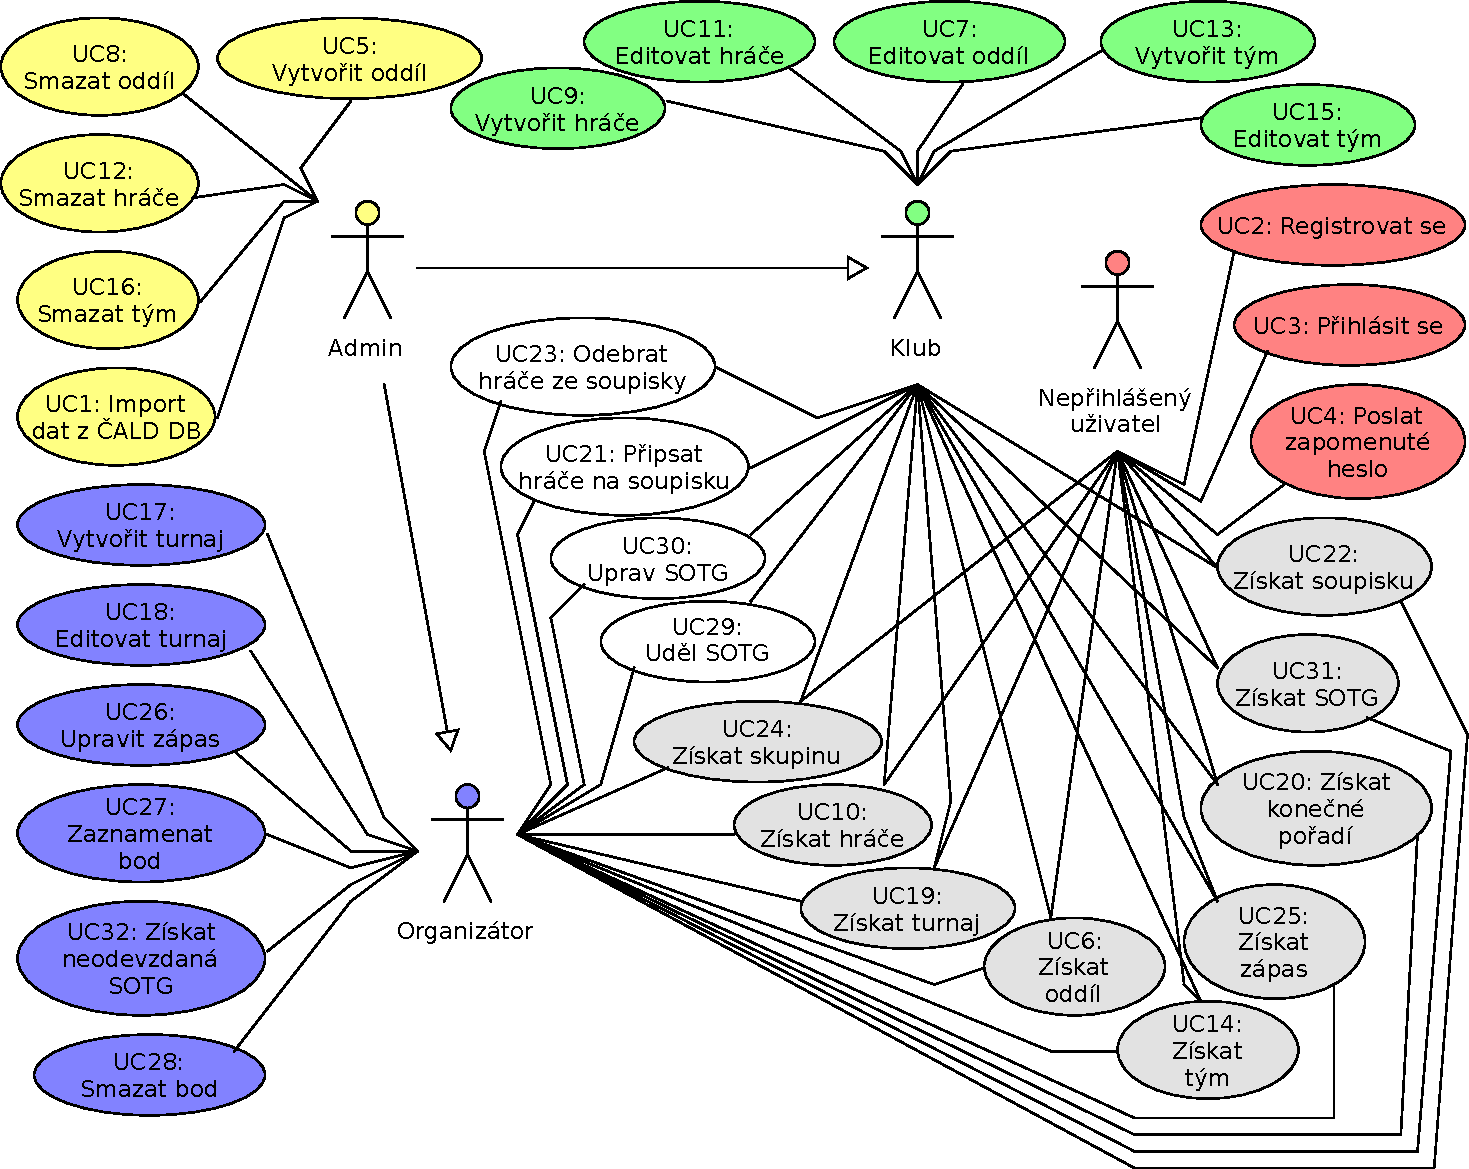
\includegraphics[width=130mm]{./images/use-case.pdf}
\caption{Use case diagram\label{overflow}}
\end{figure}

 
\chapter{Analýza}

Jelikož původní záměr zněl rozšířit mobilní aplikaci Catcher,
měli bychom se v této kapitole zabývat jejím průzkumem. Neopomene ani jiné podobné projekty.
V druhé části se podíváme na možnosti našeho řešení.

\section{Existující řešení}

\subsection*{Mobilní aplikace Catcher}

V roce 2013~\cite{cald_catcher} byla zveřejněna první verze této aplikace pro mobilní telefony s operačním systémem Android.
Autory jsou dva aktivní hráči Jiří Voseček a Ondřej Burkert. Aplikace si od svého vzniku získala velkou popularitu
ve~frisbee komunitě a dnes je používaná na většině českých turnajů. Umí zadávat výsledky
zápasů včetně podrobného průběhu bodů, rozhodovat o umístění v základních skupinách, počítat statistiky hráčů,
odevzdávat a zveřejnit vzájemná hodnocení SOTG týmů na~turnaji. Dokáže omezeně importovat oficiální soupisky týmů
na nadcházející turnaje spadající pod Českou asociaci létajícího talíře.

Kromě mobilní aplikace Catcher byl vytvořen backend v PHP~\cite{php}, který ukládá a počítá data na serveru. Ten však není
objektově orientovaný a~všechna jeho eventuální rozšíření jsou velmi náročná.

\subsubsection*{Výhody}
\begin{itemize}
  \item Backend je využíván webovou aplikací (frisbee.cz) a mobilní aplikací na~OS~Android.
  \item Přes webový prohlížeč lze přistupovat k emulátoru aplikace.
  \item Systém je již mezi organizátory turnajů zaběhnutý a na Google Play
    \footnote{Online distribuční služba, kde jsou k dispozici aplikace pro mobilní telefony a tablety s OS Android}
    má již více než 1000 stáhnutí~\cite{catcher_play}.
  \item Umí importovat soupisky na oficiální turnaje ČALD.
\end{itemize}

\begin{figure}[ht!]
\centering
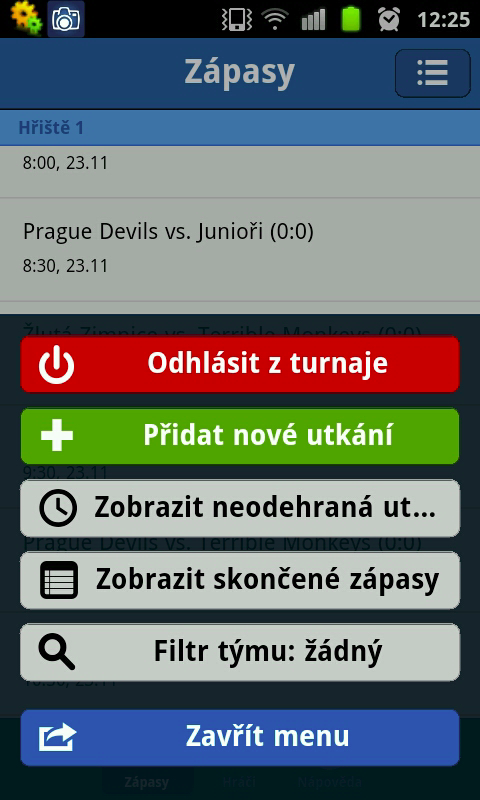
\includegraphics[width=60mm]{./images/catcher.png}
\caption{Mobilní aplikace Catcher~\cite{catcher_play}\label{overflow}}
\label{fig:uwsgi}
\end{figure}

\subsubsection*{Nevýhody}
\begin{itemize}
  \item Import soupisek z databáze ČALD je pouze poloautomatický. Administrátor musí před každým turnajem
    import spustit a zkontrolovat, zda se data uložily validně. Tomuto stavu nepřispívá ani fakt,
    že databáze ČALD, ze které se import provádí, je velmi špatně navržena.
  \item Nedisponuje žádným rozhraním, které by mohly používat další klientské aplikace.
  \item Automaticky nedoplňuje týmy v zápasech play-off do dalších kol (např. vítěze semifinále do finále apod.).
  \item Při vytváření turnaje neprobíhá žádná kontrola validity dat.
    Lze tak vytvořit spoustu chybných utkání, které se pak musí opravovat. 
\end{itemize}

\subsection*{Ultimate Organizer}

Aplikace zveřejněná v roce 2004~\cite{ultimate_organizer}, napsaná v PHP a používaná na velkých akcích jako mistrovství světa nebo Evropy
pro sledování výsledků a statistik. Poskytuje tvorbu a správu turnajů, týmů, hráčů,
výsledků, rozpisů atd. Podporuje vícejazyčnost, tisk rozpisů v PDF, přístup pro mobilní telefony
a~spoustu dalších vlastností. Dokáže zobrazit podrobné detaily o průběhu zápasů.

\subsubsection*{Výhody}
\begin{itemize}
  \item Rozsáhlá aplikace poskytující nepřeberné množství možností.
  \item Aplikace již má za sebou více než 10 let fungování.
  \item Poskytuje přístup pro mobilní telefony s webovým prohlížečem.
\end{itemize}

\subsubsection*{Nevýhody}
\begin{itemize}
  \item Nefunguje jako webová aplikace. Uživatel si musí stáhnout zdrojové kódy a aplikaci si sám nasadit na svém počítači nebo serveru.
  \item Neposkytuje žádné rozumné rozhraní, tudíž pro ni nelze vytvořit žádného klienta.
  \item Nelze sledovat dlouhodobější statistiky napříč týmy a hráči. Všechny výsledky se týkají pouze jednoho konkrétního turnaje.
\end{itemize}

\subsection*{Ultimate Central}

Webová aplikace~\cite{ultimate_central}, která slouží především ke správě soupisek na~turnajích. Pořadatel turnaje vytvoří událost
v kalendáři a zapíše všechny účastnící se týmy. Ty pak musí odevzdat svoje soupisky a potvrdit náležité dokumenty,
které jsou na~některých turnajích povinností (např. zřeknutí se možnosti žalovat organizátora aj.).
Kromě toho dokáže ukládat výsledky zápasů a hodnocení SOTG. 

\begin{figure}[ht!]
\centering
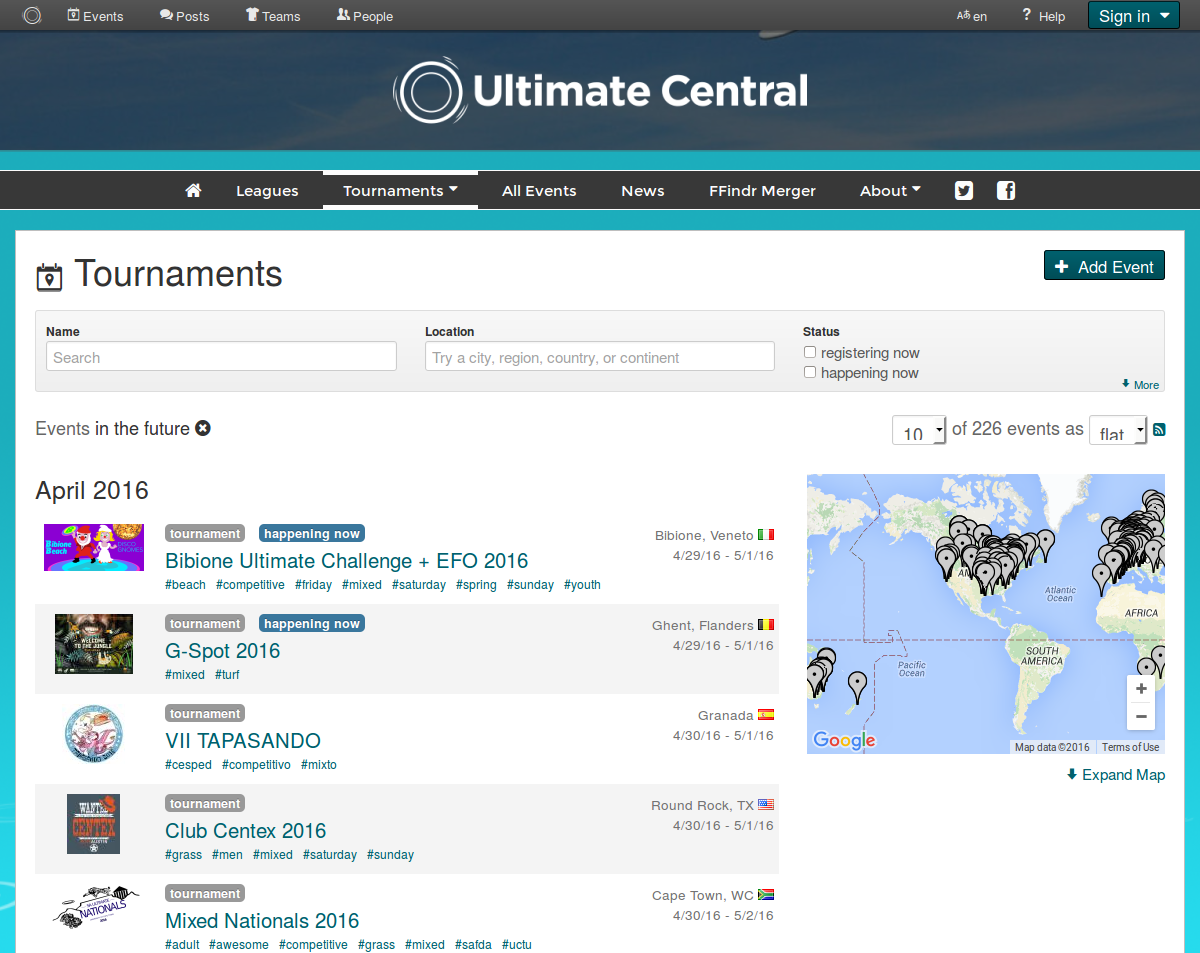
\includegraphics[width=130mm]{./images/ultimate-central.png}
\caption{Webová aplikace Ultimate Central\label{overflow}}
\end{figure}

\subsubsection*{Výhody}
\begin{itemize}
  \item Umožňuje vytvořit jednoduchou webovou stránku pro každý turnaj, na~které lze shrnout důležité informace pro všechny účastníky.
  \item Aplikace je dostupná ve webovém prohlížeči.
\end{itemize}

\subsubsection*{Nevýhody}
\begin{itemize}
  \item Neslouží ke statistikám. Do systému se zapisují pouze výsledky a hodnocení SOTG.
  \item Vyžaduje registraci a přihlašení každého jednotlivého hráče na turnaji.
  \item Stejně jako obě předchozí aplikace neposkytuje rozhraní, které by mohla využít například mobilní aplikace.
\end{itemize}

\subsection{Výsledek}

Průzkum existujících řešení naznačil, že náš projekt má smysl. Stále chybí aplikace,
která by byla zároveň plně automatizovaná (před započetím turnaje se vytvoří rozpis a~ten se
již doplňuje na základě zadaných výsledků), měla rozhraní pro libovolné tenké klienty
a~dokázala využít data z~databáze ČALD.

\section{Možnosti řešení}

Protože už od počátku známe požadavek na možnost připojení klienta v~podobě mobilní nebo webové aplikace,
je nutné poskytnout žadatelům o~přístup rozhraní, které dostatečně pokryje jejich požadavky.
Z úvodní kapitoly víme, že webová služba se dělí na dva typy - SOAP a REST.

\subsection{SOAP}

Protokol SOAP (\textit{Simple Object Access Protocol}) vystavuje aplikační logiku jako službu
a~je proveden v~syntaxi jazyka XML~\cite{xml}. Výhodou standartního značkovacího jazyka je jeho rozšíření
a značná podpora ve většině programovacích jazycích. Syntaxe XML je pro člověka relativně čitelná,
protože bývá zdlouhavá, avšak počítač musí parsování dat věnovat více času i paměti.

Nevýhodou je nestálost prostředí. Ve chvíli, kdy dojde v~SOAP API ke~změ\-ně, klient může přestat pracovat,
protože si nemusí umět poradit s odpovědí, přesněji s novou strukturou přijímaného XML souboru.
Podobně je potřeba upravovat při změnách API i strukturu požadavku.

% IDEA: Moznost napsat vice o SOAP, napriklad vlozit nejakou ukazku.
% SOAP služby standartně obsahují v URL nějaké sloveso (např. zobrazInfo).
 
\subsection{REST}

Protokol REST (\textit{Representational State Transfer}) je architektonický styl návrhu API popsaným Royem Fieldingem \cite{fielding}.
Je založený na vystavování a jednotném přístupu ke~zdrojům\footnote{resources}, kterými jsou určitá data.
Přistupuje se k~nim pomocí HTTP metod GET, POST, DELETE a PUT.

RESTová služba používá pro přenos dat řadu formátů, nejstandartnějšími jsou XML a JSON~\cite{json}.
JSON je datově méně náročnější a stejně jako XML je podporován v mnoha programovacích jazycích.

\subsubsection*{Zdroj}

Architektonický styl REST je postaven na základním prvku -- zdroji. Jde o~logický objekt,
který lze vyjádřit smysluplnou reprezentací, a~s~kterém lze manipulovat pomocí zpřístupněných metod.
Každý zdroj má svůj unikátní identifikátor URI\footnote{Uniform Resource Identifier}.

\subsubsection*{Požadavky na RESTové rozhraní}

Aby se mohlo nějaké aplikační rozhraní požadovat za RESTové (tzv. RESTful),
musí splňovat několik základních předpokladů definované Fieldingem \cite{fielding}.
Nyní si uvedeme ty nejdůležitější:

\begin{description}
    \item[Architektura klient-server]
    Rozděluje zodpovědnost mezi různé části. Klientské aplikace se nemusí starat o správu dat a server o jejich prezentaci.
    Z toho vyplývá možnost vývíjet obě kompomenty (klient a server) nezávisle na sobě.
    \item[Bezstavovost]
    Aplikační stav je udržován na straně klienta. Všechny požadavky tak obsahují pouze informace nutné k jeho zpracování.  
    \item[Jednotné rozhraní]
    Pomocí unikátního identifikátoru lze získat reprezentaci nebo manipulovat s libovolným zdrojem.
    Klient musí být schopen s daným zdrojem manipulovat na základě jeho reprezentace. Zprávy by měly být dostatečně popisné.
\end{description}

\subsection{Shrnutí}

Z předcházejícího srovnání je patrné, že na flexibilní v budoucnu rozšiřitelné rozhraní se spíše hodí REST.
Klienti nebudou tolik nachylní na úpravy API a~navíc jim bude možné data poskytnout ve~formátu JSON,
který se pro~jejich přenos hodí daleko více. XML je přece jenom spíše jazyk než formát dat.

\chapter{Návrh}

Kdybychom navrhovali SOAP službu, vzali bychom všechny případy užití (use cases) a~k~nim vytvořili
konkrétní metody. V REST je návrh trochu složitejší.
Musíme nejprve identifikovat všechny zdroje, se kterými se bude pracovat, a~umožnit
k~nim přístup pomocí standardizovaných metod. V návrhu vycházíme ze tří ustálených modelů:

\begin{itemize}
\item doménový model
\item datový model
\item use case diagramy
\end{itemize}

První dva modely nám slouží k identifikování jednotlivých zdrojů.
Doménový model poskytuje klíčové entity a vztahy mezi nimi.
Jde o~vysoko-úrovňový pohled na problematiku. Nezbytné detaily dořešíme pomocí datového modelu. 
Akce, které nejdou pokrýt pomocí standardních metod manipulujících se zdroji, nám mohou poskytnout use case diagramy.
My si vystačíme s případy užití a jejich diagramem, který jsme zpracovali v sekci~\ref{sec:use_case}. 
Diagramy všech tří modelů jsou tedy v této práci zpracovány.

\subsection{Doménový model}

Tvorba doménového modelu (na obrázku~\ref{fig:domain_model}) vychází ze zadání. Obsahuje následující entity,
jež modelují základní představu o systému.

\begin{figure}[ht!]
\centering
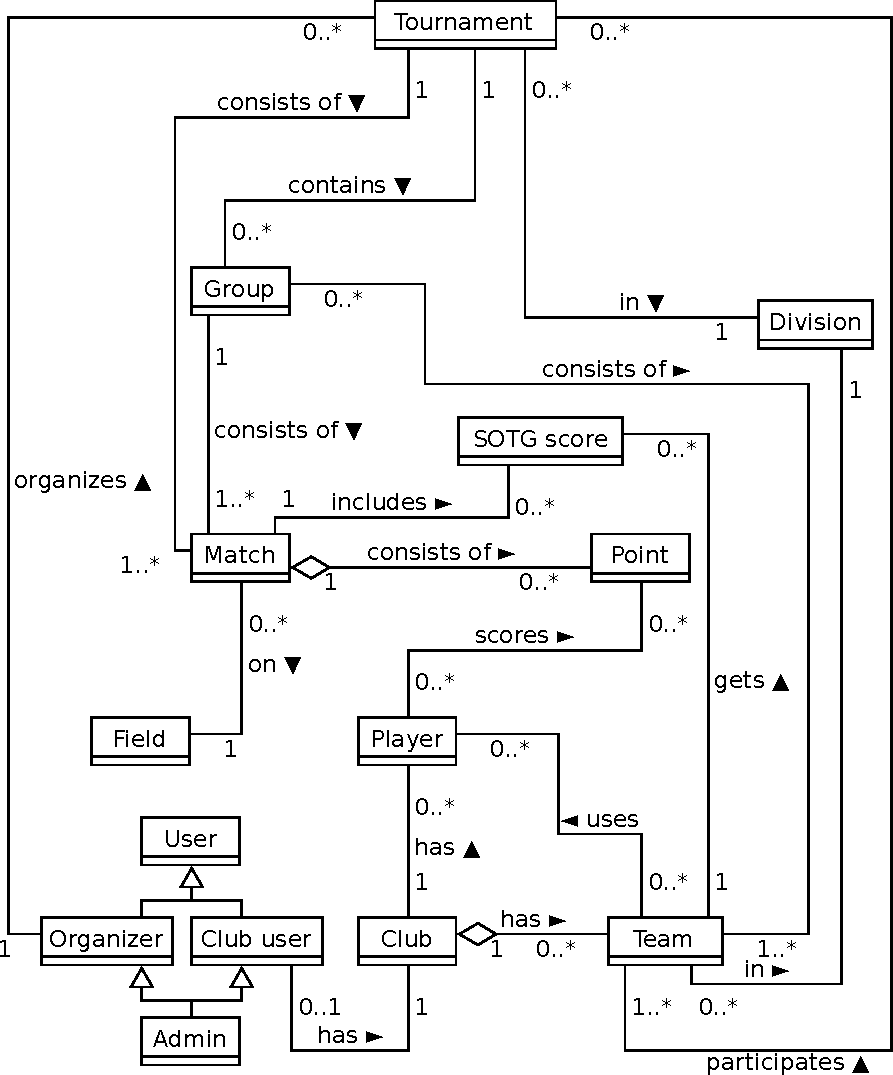
\includegraphics[width=130mm]{./images/domenovy-model.pdf}
\caption{Doménový model\label{overflow}}
\label{fig:domain_model}
\end{figure}


\begin{description}
  \item[Uživatel (user)]
  Uživatel je identifikován e-mailem a heslem nebo tokenem (více v sekci~\ref{sec:security}).
  Zároveň disponuje jednou ze tří rolí (\texttt{club}, \texttt{organizer} a~\texttt{admin}).
  \item[Oddíl (club)]
  Oddíl je logický prvek, který zastřešuje více týmů. Správu oddílu provádí klubový účet.
  \item[Tým (team)]
  Tým je vázán na oddíl. Jeho identifikátory jsou divize a stupeň týmu (např. A-tým).
  \item[Divize (division)]
  Kategorie, ve které se pořádají turnaje, nebo je složen tým. Například juniorská divize. % Například ženský tým je v divizi \texttt{women}.
  \item[Turnaj (tournament)]
    Turnaj může nabývat několika stavů (stavový diagram na~obrázku~\ref{fig:state_tournament}).
    Po vytvoření turnaje lze až do potvrzení (příznak \texttt{ready}) měnit týmy, které se turnaje zúčastní.
    Po něm mohou klubové účty odevzdávat soupisky za svoje týmy a na turnaji je možné aktivovat zápasy. Ve chvíli,
    kdy všechny týmy odevzdají svoje hodnocení SOTG a je známo finální pořadí týmů,
    lze turnaj ukončit (příznak \texttt{terminated}). Do~té~doby skryté výsledky hodnocení SOTG se stanou veřejnými.
    Turnaj je spravován administrátorem nebo uživatelem s rolí \texttt{organizer} (tzv.~organizátor).
    \begin{figure}[ht!]
      \centering
      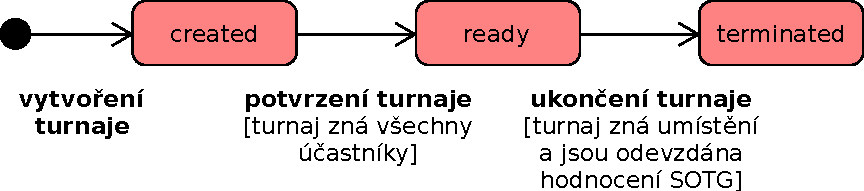
\includegraphics[width=110mm]{./images/stavovy-diagram-turnaj.pdf}
      \caption{Stavový diagram turnaje\label{overflow}}
      \label{fig:state_tournament}
    \end{figure}
  \item[Zápas (match)]
    Zápas má, stejně jako turnaj, tři stavy (obrázek~\ref{fig:state_match}). Akti\-vováním zápasu je umožněno zadat konečný výsledek
    nebo postupně vkládat jednotlivé body. Ukončením (příznak \texttt{terminated}) se konečný výsledek uloží a~následně se promítne
    v dalším postupu turnajem (vítězný tým posune do dalšího zápasu, týmům se přidá výhra ve skupině~apod.).
    \begin{figure}[ht!]
      \centering
      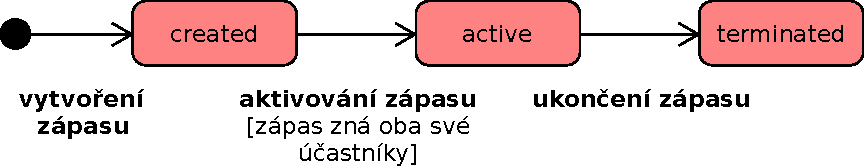
\includegraphics[width=110mm]{./images/stavovy-diagram-zapas.pdf}
      \caption{Stavový diagram zápasu\label{overflow}}
      \label{fig:state_match}
    \end{figure}
  \item[Bod (point)]
    Zápas je složen z několika bodů. Každý bod je záznamem o~skórování. Uchovává informaci, jaký hráč a komu nahrával.
    Zápas může být ukončen i bez jednotlivých bodů zadáním konečného skóre.
  \item[Skupina (group)]
    Jde o několik týmů, které hrají zápasy pouze mezi sebou. Po odehrání všech utkání ve skupině se podle pravidel určí pořadí a~na~jeho základě se týmy posunou turnajem dál.
  \item[Hřiště (field)]
    Zápas se musí někde hrát. K tomu slouží hřiště.
  \item[Hodnocení SOTG (SOTG score)]
    Po každém utkání musí tým ohodnotit soupeře hodnocením Spirit of the Game. Zjednodušeně jde o~číselné vyjádření na~stupnici od~0 do 20.
\end{description}

\subsection{Datový model}

Pro ujasnění entit a vazeb mezi nimi byl vhodný doménový model. Jeho konkrétní implementací je model datový.
Ten je dekomponován, tj. zbaven M:N~vazeb, a~oproti doménovému modelu obsahuje nové
(relační) objekty včetně atributů. Kompletní datový model je dostupný v příloze~\ref{appendix:data_model}.

\section{Identifikace zdrojů}

Abychom mohli namapovat zdroje na konkrétní URI\footnote{Uniform Resource Identifier},
musíme je nejprve jedno\-značně určit. Mnoho programátorů zde postupuje tak, že vychází
z~datového modelu a~použije prosté mapování \textit{tabulka = zdroj}.
Návrh je sice rychlý, ale nemusí být dostatečný. Navíc vytváří příliš těsnou vazbu mezi interní datovou reprezentací
a~logickou strukturou zdrojů. Zdroje v této práci vycházejí z doménového modelu.

\subsection{Základní typy zdrojů}

Podle~\cite{rest_vse} se zdroje dělí na tři základní typy:

\begin{description}
  \item[Dokument] Reprezentace jednoho konkrétního zdroje v určitém formátu.
  \item[Kolekce] Množina zdrojů stejného typu. Jedná se o skupiny samostatných entit.
  \item[Kontroler] Nezávislé metody aplikace. Akce, které nelze vyjádřit pomocí standardních
  CRUD\footnote{Create, Read, Update, Delete - vytváření, čtení, úpravy a mazání} metod HTTP protokolu.
\end{description}

\subsection{Návrh URI}

Návrh se týká cesty v hierarchické části URI. Pro udržení kvality je doporučené se při návrhu držet několika zásad. Cesta by podle~\cite{rest_vse} měla:
    
\begin{itemize}
\item mít konzistentní a logickou strukturu
\item mít dobře znázorněnou hierarchickou strukturu
\item být nezávislá na zvolené technologii
\item transparentně používat HTTP metody a kódy
\item používat:
\begin{itemize}
\item jednotná čísla pro označení konkrétních zdrojů
\item množná čísla pro kolekce
\item slovesa pro kontrolery
\end{itemize}
\end{itemize}

\begin{figure}[ht!]
  \centering
  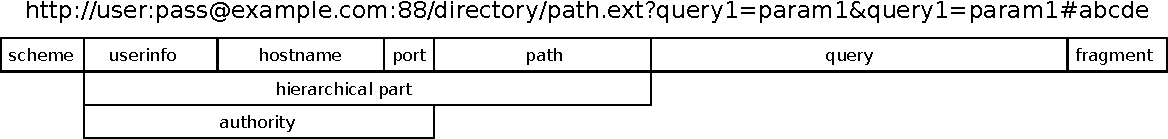
\includegraphics[width=130mm]{./images/uri.pdf}
  \caption{Jednotlivé komponenty URI; zdroj: autor na základě~\cite{uri}\label{overflow}}
\end{figure}

S těmito zásadami byl vytvořen následující návrh na mapování operací, které lze provádět nad zdroji.
Identifikátor značíme \texttt{\{id\}} nebo \texttt{\{ide\}} (druhý identifikátor je textový).
V cestách je vynechán prefix \texttt{/api}, který odděluje aplikační a dokumentační část.

\begin{itemize}
  \item \texttt{\textbf{/login}}
  \begin{itemize}
    \item \textbf{popis:} Přihlašuje uživatele. Po přihlášení vrátí přístupový token (více v sekci~\ref{sec:security}).
    \item \textbf{metoda:} POST
    \item \textbf{pokrývá:} UC3
  \end{itemize}
  \item \texttt{\textbf{/forgotten-password}}
  \begin{itemize}
    \item \textbf{popis:} Odešle nové náhodně vygenerované heslo na e-mail uživatele.
    \item \textbf{metoda:} POST
    \item \textbf{pokrývá:} UC4
  \end{itemize}
  \item \texttt{\textbf{/users}}
  \begin{itemize}
    \item \textbf{popis:} Slouží k vytváření nových uživatelů.
    \item \textbf{metoda:} POST
    \item \textbf{pokrývá:} UC2
  \end{itemize}
  \item \texttt{\textbf{/user/\{id\}}}
  \begin{itemize}
    \item \textbf{popis:} Spravuje konkrétního uživatele. Lze mu nastavit nový e-mail nebo~heslo.
    \item \textbf{metoda:} PUT
    \item \textbf{pokrývá:} UC21
  \end{itemize}
  \pagebreak
  \item \texttt{\textbf{/clubs}}
  \begin{itemize}
    \item \textbf{popis:} Kolekce oddílů.
    \item \textbf{metoda:} GET, POST
    \item \textbf{pokrývá:} UC5, UC6
  \end{itemize}
  \item \texttt{\textbf{/club/\{id\}}}
  \begin{itemize}
    \item \textbf{popis:} Operace nad konkrétním oddílem. Možnost uložit město a~zemi původu.
    \item \textbf{metoda:} GET, PUT, DELETE
    \item \textbf{pokrývá:} UC6, UC7, UC8
  \end{itemize}
  \item \texttt{\textbf{/club/\{id\}/players}}
  \begin{itemize}
    \item \textbf{popis:} Kolekce všech klubových hráčů.
    \item \textbf{metoda:} GET
    \item \textbf{pokrývá:} UC10
  \end{itemize}
  \item \texttt{\textbf{/club/\{id\}/teams}}
  \begin{itemize}
    \item \textbf{popis:} Kolekce všech týmů, které zastřešuje konkrétní oddíl.
    \item \textbf{metoda:} GET
    \item \textbf{pokrývá:} UC14
  \end{itemize}
  \item \texttt{\textbf{/players}}
  \begin{itemize}
    \item \textbf{popis:} Kolekce hráčů.
    \item \textbf{metoda:} GET, POST
    \item \textbf{pokrývá:} UC9, UC10
  \end{itemize}
  \item \texttt{\textbf{/player/\{id\}}}
  \begin{itemize}
    \item \textbf{popis:} Operace nad konkrétním hráčem.
    \item \textbf{metoda:} GET, PUT, DELETE
    \item \textbf{pokrývá:} UC10, UC11, UC12
  \end{itemize}
  \pagebreak
  \item \texttt{\textbf{/teams/}}
  \begin{itemize}
    \item \textbf{popis:} Kolekce týmů.
    \item \textbf{metoda:} GET, POST
    \item \textbf{pokrývá:} UC13, UC14
  \end{itemize}
  \item \texttt{\textbf{/team/\{id\}}}
  \begin{itemize}
    \item \textbf{popis:} Operace nad konkrétním týmem.
    \item \textbf{metoda:} GET, PUT, DELETE
    \item \textbf{pokrývá:} UC14, UC15, UC16
  \end{itemize}
  \item \texttt{\textbf{/divisions}}
  \begin{itemize}
    \item \textbf{popis:} Kolekce divizí.
    \item \textbf{metoda:} GET
  \end{itemize}
  \item \texttt{\textbf{/tournaments}}
  \begin{itemize}
    \item \textbf{popis:} Kolekce turnajů, kterou lze filtrovat pomocí pěti různých parametrů.
    \item \textbf{metoda:} GET, POST
    \item \textbf{pokrývá:} UC17, UC19
  \end{itemize}
  \item \texttt{\textbf{/tournament/\{id\}}}
  \begin{itemize}
    \item \textbf{popis:} Správa turnaje. Možnost turnaji upravit příznaky \texttt{ready} a~\texttt{terminated}.
    \item \textbf{metoda:} GET, PUT
    \item \textbf{pokrývá:} UC18, UC19
  \end{itemize}
  \item \texttt{\textbf{/tournament/\{id\}/standings}}
  \begin{itemize}
    \item \textbf{popis:} Zobrazuje výsledné pořadí týmů na turnaji, včetně kategorie SOTG.
    \item \textbf{metoda:} GET
    \item \textbf{pokrývá:} UC20
  \end{itemize}
  \item \texttt{\textbf{/tournament/\{id\}/players}}
  \begin{itemize}
    \item \textbf{popis:} Slouží pro správu soupisek na turnaji.
    \item \textbf{metoda:} GET, POST, DELETE
    \item \textbf{pokrývá:} UC21, UC22, UC23
  \end{itemize}
  \pagebreak
  \item \texttt{\textbf{/tournament/\{id\}/teams}}
  \begin{itemize}
    \item \textbf{popis:} Slouží pro správu týmů na turnaji.
    \item \textbf{metoda:} GET, PUT
  \end{itemize}
  \item \texttt{\textbf{/tournament/\{id\}/matches}}
  \begin{itemize}
    \item \textbf{popis:} Kolekce zápasů, kterou lze filtrovat pomocí šesti různých parametrů.
    \item \textbf{metoda:} GET
    \item \textbf{pokrývá:} UC25\\
  \end{itemize}
  \item \texttt{\textbf{/tournament/\{id\}/groups}}
  \begin{itemize}
    \item \textbf{popis:} Kolekce skupin.
    \item \textbf{metoda:} GET
    \item \textbf{pokrývá:} UC24
  \end{itemize}
  \item \texttt{\textbf{/tournament/\{id\}/group/\{ide\}}}
  \begin{itemize}
    \item \textbf{popis:} Konkrétní skupina.
    \item \textbf{metoda:} GET
    \item \textbf{pokrývá:} UC24
  \end{itemize}
  \item \texttt{\textbf{/tournament/\{id\}/spirits}}
  \begin{itemize}
    \item \textbf{popis:} Kolekce všech hodnocení SOTG. Možnost filtrovat hodnocení pro jeden konkrétní tým.
    \item \textbf{metoda:} GET
    \item \textbf{pokrývá:} UC31
  \end{itemize}
  \item \texttt{\textbf{/tournament/\{id\}/missing-spirits}}
  \begin{itemize}
    \item \textbf{popis:} Seznam týmů, které hodnocení SOTG neodevzdaly.
    \item \textbf{metoda:} GET
    \item \textbf{pokrývá:} UC32
  \end{itemize}
  \item \texttt{\textbf{/match/\{id\}}}
  \begin{itemize}
    \item \textbf{popis:} Správa utkání.
    \item \textbf{metoda:} GET, PUT, 
    \item \textbf{pokrývá:} UC25, UC26
  \end{itemize}
  \pagebreak
  \item \texttt{\textbf{/match/\{id\}/points}}
  \begin{itemize}
    \item \textbf{popis:} Zobrazuje detailní popis zápasu. Konkrétně jeho odehrané body seřazené chronologicky.
      Dále poskytuje ukládání nových bodů a úpravu stávajících (například změna hráče, který skóroval).
    \item \textbf{metoda:} GET, POST, PUT, DELETE
    \item \textbf{pokrývá:} UC25
  \end{itemize}
  \item \texttt{\textbf{/match/\{id\}/spirits}}
  \begin{itemize}
    \item \textbf{popis:} Vrátí detail jednoho zápasu včetně hodnocení SOTG obou týmů. Kromě toho umožňuje odevzdat hodnocení SOTG.
    \item \textbf{metoda:} GET, POST, PUT
    \item \textbf{pokrývá:} UC25, UC29, UC30
  \end{itemize}
\end{itemize}

\chapter{Implementace}

\section{Výběr technologií}

\indent

V době, kdy existuje obrovské množství programovacích jazyků, jejich ekosystémů a dalších frameworků je důležité se umět nespálit. 
Vybrat špatné technologie totiž může znamenat prodloužení vývoje, zvýšení celkových nákladů nebo dokonce ukončení projektu.
Proto je nutnost tuto část dostatečně analyzovat a svědomitě zvážit, aby nedošlo k omylu, který by zabraňoval úspěšné dokončení.
Pro adekvátní výběr tak bylo potřeba specifikovat příslušná kritéria, které by jasně porovnala všechny zvažované technologie:

\subsubsection*{Podpora webových služeb}
Při tvorbě webové aplikace nemůže být ani řeč o technologii, která by pro použití na webu nebyla vhodná. Technologie musí
umět pracovat s mapováním URL a HTTP metod na zdroje a pracovat s běžnými formáty dat v internetové komunikaci (např. JSON).

\subsubsection*{Dokumentace a uživatelská podpora}
Pro pochopení technologie a její správné používání je často potřeba znát detaily, které se uživatel dozví z dokumentace.
Ta dokáže často výrazně zkrátit učící křivku a programátorovi tak šetří čas. Pokud dokumentace nestačí, může často její
nedostatky zachránit dostatečně široká uživatelská základna. Velká uživatelská podpora navíc snižuje riziko zestárnutí zvolené technologie.

\subsubsection*{Znalost technologie}
Pokud již programátor některou z technologií zná, může mu tato znalost ušetřit mnoho času při vývoji. Nemusí totiž novou technologii
nijak složitě zavádět nebo se učit její použití. Vhodným výběrem se také může vyvarovat situacím, kdy až v průběhu implementace narazí
na neřešitelné problémy. Zavrhnout neznámé technologie ale může znamenat přijít o možnost používat nástroje, které jsou problémům šité na míru. 

\subsubsection*{Výkon}
I když aplikace nepočítá s vetším provozem čítající stovky požadavků za sekundu, není důvod používat technologie, které jsou pomalé
nebo spotřebovávají příliš moc prostředků.

\section{Zvolené technologie}

\subsection{Programovací jazyk Python}

\indent

Python je víceúčelový skriptovací jazyk navrhnut v roce 1991 \cite{python-year} Guido van Rossumem.
Je vyvíjen jako open source projekt a je bezplatně dostupný pro většinu dostupných platforem (Unix, Windows, Mac OS).
V distribucích Linuxu je často součástí základní instalace. Díky velkému množství knihovních modulů z různých oblastí
má velice široké možnosti uplatnění. Běžně jej používají ve firmách jako Google, Dropbox, YouTube, Red Hat, Cisco,
Facebook nebo Microsoft \cite{python-companies}.

\medskip

Protože jde o dynamický interpretovaný jazyk, jeho zdrojový kód není nutné překládat překladačem do strojového kódu.
Je to zárovéň hybridní jazyk, protože umožňuje používat různá programovací paradigmata, včetně objektově orientovaného,
imperativního, procedurálního nebo v omezené míře i funkcionálního. I když je Python mnohokrát označován za skriptovací jazyk,
jeho návrh umožňuje psaní rozsáhlých a plnohodnotných aplikací včetně GUI. Podporuje také dynamickou kontrolu datových typů.

\medskip

Je to jazyk, který se velmi snadno učí a bývá považován za jeden z nejvhodnějších programovacích jazyků pro začátečníky.
Pomáhá tomu jeho jednoduchá syntaxe a čistota kódu. Na rozdíl od jiných jazyků bývá jeho zdrojový kód často krátký a dobře čitelný.
Je tak vhodný pro výuku i využití v praxi. Podle PYPL indexu\footnote{PopularitY of Programming Language Index je vytvořen analyzováním toho,
jak často jsou tutoriály jednotlivých programovacích jazyků hledány na Googlu.} je Python celosvětově nejrychleji roustoucí programovací jazyk
v~oblíbenosti za posledních pět let \cite{python-pypl}.
V dubnovém žebříčku roku 2016 drží druhé místo mezi jazyky Java a PHP. Mnoho dalších žebříčků pak uvádí Python vždy v prvních pěti místech.

\medskip

Po stránce výkonu je na tom Python relativně dobře, protože mnoho na~výkon náročných knihoven je implementováno v~jazyce C.
V porovnání s ostatními interpretovanými jazyky je na tom samotný Python taky dobře.
Fakt se kterým ale musíme počítat je ten, že dynamicky interpretované jazyky jsou obecně pomalejší, než kompilované jazyky.

\subsection{Webový framework Falcon}

% TODO: dovysvetlit, co je to UWSGI, mozna dat pred Falcon 

\indent

Falcon je minimalistický webový framework pro vývoj aplikačních backendů a jejich API s otevřeným zdrojovým kódem,
populární pro svoji neuvěřitelnou rychlost. Falcon ctí architektonický styl REST, což znamená, že mapuje použité
zdroje a jejich metody do HTTP protokolu.

\medskip

Falcon disponuje minimálním množstvím závislostí na jiných knihovnách a díky jeho flexibilitě je ho možné
používat ve většině verzích Pythonu\footnote{Vývoj v Pythonu poznamenalo v roce 2008 vydání nové verze Python 3.0,
která je částečně zpětně nekompatibilní.}. Kromě toho umí pracovat s WSGI. Nevýhodou Falconu je menší uživatelská
základna na rozdíl od konkurenčního Flasku, jenž patří mezi nejpopulárnější webové frameworky pro Python.

\begin{table}[htb]
 \centering
 \begin{tabular}{|l||c|c|c|c|}\hline
 \bfseries \bfseries framework & \bfseries req/sec & \bfseries $\mu$s/req & \bfseries výkon \\[2mm]
 \hline
 Falcon (0.3.0) & 21,858 & 46 & 8x \\
 \hline
 Bottle (0.12.8) & 12,583 & 79 & 4x \\
 \hline
 Werkzeug (0.10.4) & 4,708 & 212 & 2x \\
 \hline
 Pecan (0.8.3) & 3,442 & 291 & 1x \\
 \hline
 Flask (0.10.1) & 2,837 & 352 & 1x \\
 \hline
 \end{tabular}
 \caption{Výkonnostní test několika podobných webových frameworků pro~CPython~2.7.9 \cite{falcon-benchmarks}. Jde o~implementaci jazyka Python, kterou používá Catcher.}
\end{table}

\subsection{Databáze MySQL}

\indent

Relační datábáze, se kterou probíhá komunikace pomocí jazyka SQL, jak už název napovídá.
Díky svému výkonu, snadné použitelnosti (lze ji nainstalovat na Linux, Windows, OS X a další) a faktu,
že jde o volně šiřitelný software (je k dispozici i pod komerční licencí),
je MySQL velmi populární. Je součástí velmi oblíbené kombinace
základního softwaru na serverech známou pod zkratkou LAMP\footnote{Linux, Apache, MySQL, PHP}.

\medskip

Pro správu databáze se používá zpravidla příkazový řádek nebo lze separátně stáhnout
a nainstalovat nástroj zvaný MySQL Workbench. Ten byl použit i v této práci při návrhu databázového modelu.
Od svého vzniku v roce 1995 [ZDROJ] se od MySQL odpojilo několik alternativních větví (tzv. fork).
Mezi nejznámější případy patří MariaDB [ZDROJ] a Percona [ZDROJ].

\subsection{Peewee ORM}

\indent

Peewee je implementace ORM pro jazyk Python. Obsahuje podporu pro~databáze SQLite,
PostgreSQL a~MySQL. Je otevřeným softwarem a jeho zdrojový kód je dostupný na~GitHubu.

\subsubsection{Co je to ORM?}

\indent

ORM (\textit{Object-relational mapping}) je programovací technika, která zajišuje, že data z relační databáze
se automaticky konvertují do objektů v OOP. Programátor tak pracuje s perzistentními objekty,
místo psaní SQL dotazů. Pokročilejší ORM dokonce dokážou využít objektovou dědičnost, což relační databáze nepodporují.

\medskip

Technika je často kritizována, protože jde často o zbytečnou režii navíc
a programátory odnaučuje psát SQL dotazy, navíc efektivně.
Mnoho ORM nástrojů složitější dotazy přeloží do jazyka SQL tak neúčinně,
že dotaz může být mnohonásobně pomalejší, než kdyby je programátor napsal v SQL sám.
V závěru této práce jsem použití ORM zhodnotil.

\subsection{Verzovací systém Git}

\indent

Git je nástroj vytvořený Linusem Torvaldem (tvůrcem Linuxového jádra).
Slouží k distribuované správě verzí libovolných digitálních informací, například zdrojových kódů.
Výraznou výhodou je možnost spolupráce velkého množství programátorů na jednom softwarovém projektu. 
Každý programátor má adresář s projektem na svém lokálním disku a všechny změny sdílí s centrálním repozitářem,
ke kterému mají přístup i všichni ostatní programátoři. Ti si pak mohou stáhnout všechny změny,
které se na projektu staly. Git neuchovává úplný stav každé verze, ale pouze rozdíly mezi jednotlivými verzemi.
Tím výrazně šetří paměť.  

\medskip

Ruku v ruce jde s popularitou Gitu nahoru i služba GitHub.
Ta nabízí bezplatný i komerční hosting pro repozitáře softwarových projektů.
Zdarma, a díky tomu populární v dané oblasti, je GitHub pro open source projekty.
Funguje od roku 2008 a hostuje už více jak 11 miliónů repozitářů [ZDROJ].
Poskytuje mnoho dalších vlastností, jako například možnost diskutovat nad kódem
nebo zasílat notifikace o změnách.

\subsection{Webový server Nginx}

\indent

Nginx je webový server a reverzní proxy\footnote{Reverzní proxy se používá pro zvýšení výkonu webového serveru.
Rozděluje vstupující provoz na více serverů, například vyvažuje zátěž serverů zapojených v clusteru.}, který pracuje s běžnými protokoly.
První oficiální verze se objevila v roce 2004 \cite{nginx-changes}, kterou vyvynul Ruský softwarový inženýr Igor Sysoev.
Zaměřuje se na vysoký výkon a nízké nároky na pamět. Je používán velkými firmami
díky propracované možnosti rozložení zátěže. Z velkých firem je to například Netflix, Wordpress.com,
GitHub, Dropbox nebo Seznam.cz.

\medskip

Dnes je již s 25 \% druhým nejpoužívanějším webovým serverem v prvním milionu nejzatíženějších webů na světě.
Napříč celým webem je pak na třetím místě s přibližně 16 \%. I když je Apache HTTP Server stále jednička, 
jejich rozdíl se neustále zmenšuje \cite{nginx-statistic}. Nginx je open source.

% TODO: IDEA: Moznost prilozit obrazek s grafem nebo tabulkou.

\section{Adresářová struktura}

% TODO: tady se trochu vic rozepsat

\indent

Adresářová struktura popsaná v této sekci odpovídá struktuře, ve které projekt najdete na GitHubu.
Služba se dělí na dvě časti, v jedné se nachází aplikační logika a v druhé je jednoduchá webová stránka s dokumentací.

\medskip

Celou aplikační logiku najdeme v adresáři \texttt{/catcher}, kde se nachází zdroje a jejich mapování na URL,
mapování relační databáze na objekty nebo zdrojové kódy zajišťující autentizaci a autorizaci uživatelů.
Dokumentace se nachází v adresáři \texttt{/html}, kde jsou všechny důležité soubory pro použití JavaScriptu a~CSS na webu.

\medskip

Konfigurační soubory jsou uloženy v adresáři \texttt{/catcher/config}.
Nachází se zde přístupové údaje k databázím (produkční a testovací) nebo emailovému účtu pro zasílání nového hesla.
Konfigurační soubory nejsou uloženy v~repozitáři na Gitu. 

\begin{figure}[ht!]
\dirtree{%
  .1 /.\DTcomment{kořenová složka}.
  .2 /bin\DTcomment{spustitelné skripty}.
  .2 /catcher\DTcomment{aplikační logika}.
  .3 /api\DTcomment{vrstva spravující API}.
  .3 /config\DTcomment{konfigurační soubory}.
  .3 /logger\DTcomment{logování aplikace}.
  .3 /models\DTcomment{mapování relační databáze na OOP}.
  .3 /resources\DTcomment{zdroje}.
  .3 /test\DTcomment{testy}.
  .3 /restapi.py\DTcomment{spouštěcí skript}.
  .2 /html\DTcomment{adresář dostupný z webu (dokumentace)}.
  .2 /nginx\DTcomment{konfigurační soubory webového serveru}.
  .2 /sql\DTcomment{SQL skripty}.
  .2 /LICENSE\DTcomment{licence softwaru}.
  .2 /README.md\DTcomment{výčet závislostí a ostatní informace}.
  .2 /VERSION\DTcomment{aktuální verze}.
}
\caption{Struktura webové služby včetně adresáře pro webovou dokumentaci.\label{overflow}}
\end{figure}

\section{Bezpečnost}

\textit{Jak probíhá komunikace, jak se uživatelé autentizují a autorizují.}

Oauth

\section{Dokumentace}

Sphinx atd.

\section{Další}

\textit{Popíšu vybrané části systému. Například jak aplikace komunikuje s databází, nebo jak se počítají SOTG, postupy ze skupin apod. Nemám ještě dovymšlené.}

\chapter{Testování}

% IDEA: rozepsat se s rozdelenim dalsich testu

Jednou z nejdůležitejších součástí vývoje je testování. Pomáhá zkoumat funkčnost softwaru a v případě bezchybného
a úplného testování zajišťuje, že výsledná aplikace neobsahuje chyby a má požadované vlastnosti.
Testování se často provádí ve více iteracích, například pravidelně před vydáním nové verze softwaru.
Součástí testování je pak především reportování nalezených chyb.

Testy se dělí na tzv. black-box a white-box testy. Při testování černé skřínky nemáme informace o vnitřní podobě a porovnáváme
pouze správnost výstupních dat po zadání vstupních. Do testovaného subjektu se nelze podívat, vidíme jen to, jak se chová navenek.
Důvodem tohoto typu testování je analyzovat software z pohledu uživatele.
Na opačné straně se při znalosti implementace používá testování bílé skřínky. Sice tato metoda zastiňuje pohled uživatele,
ale tester je schopen lépe určit, kde hledat případné chyby. Při~částečné znalosti softwaru se ještě používá pojem testování šedé skřínky (gray-box).
Neznáme například přesnou podobu zdrojového kódu, ale jen použitý algoritmus použitý v aplikaci. 

Testy se také dělí na automatizované a manuální. Méně nákladnou a rychlejší cestou je zpravidla automatizované testování,
kdy se automaticky spouští velké množství testů, často i s velkým množstvím vstupních dat. Tyto testy se používají v místech,
kde dochází k opakování stejného nebo velmi podobného scénáře. Ne vždy se ale používá pouze automatizované testování.
Když test vyžaduje lidský úsudek, rozdílné přístupy nebo jej není nutné pravidelně opakovat, používá se manuální testování či kombinace obojího.

\section{Testování Catchera}

Testování softwaru je stále velmi podceňovaný obor a často je tato fáze vývoje odsunuta na druhou kolej nebo zcela vynechána.
Kromě toho, že psaní testů se ukázalo jako nejrychlejší způsob odhalování chyb, bylo pak ještě více překvapující, že při~použití
techniky TDD\footnote{Test-driven development - technika, kdy se testy píší ještě před samotným vývojem.} se znatelně zefektivnil
vývoj. Už~při~psaní zdrojového kódu jsem tak mohl jednoduše spouštět již vytvořené testy a znát jejich stav.
Díky specifickému popisu získání a~manipulace se zdroji v architektuře REST jsem většinu testů podřídil tomuto rozdělení a prováděl
jsem tzv. testování funkcionalit -- z pohledu uživatele, ověřování úzce zaměřených scénářů.

V Pythonu se nejrozšířenější framework pro automatizované testování jmenuje Unittest~\cite{python_unittest}. Já jsem však využil testovací nástroj, jenž přímo
poskytuje webový framework Falcon. Je potřeba zmínit, že tento nástroj většinu metod dědí od~základního Unittestu a~jeho možnosti pouze
rozšiřuje pro~lepší a~rychlejší testování REST API.

Automatizovanými testy jsou v~Catcheru pokryty všechny zdroje s~jejich metodami (celkem jich je 66). Typicky jsou testy po~několika sdružovány do~jedné třídy,
ve~které je možnost vytvořit specifické testovací prostředí. V knihovně \texttt{unittest} jsou pro tyto účely často používány metody \pythoninline{setUp()} a~\pythoninline{tearDown()},
které jsou volány před, respektive po každém testu. Důsledek tohoto chování je zajištění velmi důležitého aspektu v testování -- nezávislosti testů.
Bez něj by mohly testy pracovat nad stejnou množinou dat a navzájem si \uv{kazit} výsledky.
Nejčastější podoba testů pro~Catchera je vidět v~následující velmi zjednodušené ukázce kódu: 

\begin{python}
class TestClubs(falcon.testing.TestBase):

    def setUp(self):
      '''Spustí se před každým testem,
      zpravidla naplní testovací databázi daty.'''

    def tearDown(self):
      '''Spustí se po každém testu,
      zpravidla vyčistí testovací databázi.'''

    def testGet(self):
      '''Testuje požadavek GET - získá kolekci všech oddílů.'''     
      response = self.simulate_request('GET', '/api/clubs')
      self.assertEqual(self.srmock.status, HTTP_200)

    def testPost(self):
      '''Testuje požadavek POST - vytvoří nový oddíl.'''
      response = self.simulate_request('POST', '/api/clubs', body)
      self.assertEqual(self.srmock.status, HTTP_201)
\end{python}

Kromě porovnávání návratových HTTP kódů se v mým testech zkoumá podoba a obsah návratových dat, správné vyhazování vyjímek
nebo stav testovací databáze před a po volání metod.

\chapter{Nasazení}

K testování a provozu webové aplikace jsem získal virtualizovaný server, ke~kterému přistupuji pomocí SSH
\footnote{Program, který umožňuje komunikaci zabezpečeným protokolem. Používá TCP/IP.}.

\subsection*{Virtuální privátní server}

Jde o server běžící na virtualizovaném hardwaru, který se často označuje zkratkou VPS.
Bývá poskytován hostingovými společnostmi, které svůj fyzický stroj nabízejí více klientům najednou.
Každému zákazníkovi vymezí prostor s~vlastní instancí operačního systému, jednotlivými hostingovými službami
a~vlastní konfigurací. Nevýhodu je sdílení fyzických prostředků, poněvadž při~nedostatečném nastavení
může docházet k~ovlivňování cizích VPS. Výhodou je naopak levnější pořízení ve~srovnání s celým fyzickým serverem.

\section{Softwarové požadavky}

% TODO: zeptat se Davida na port, protoze ten port muze byt u mne zablokovany

Aplikace běží na VPS s OS Ubuntu~\cite{ubuntu} verze 15.10. Na veřejné adrese virtuálního serveru
je dostupná RESTová webová služba Catcher, s níž může zvnějšku komunikovat libovolná aplikace,
která má připojení k internetu. Jako prostředník mezi klientskou aplikací
a~uWSGI~2.0.12~\cite{python_uwsgi}, jehož úkolem je udržovat Catchera, zde běží webový server Nginx 1.9.3.
Data se ukládají na databázový server MySQL verze 5.6.28.

Pro běh aplikace byly stáhnuty všechny potřebné balíčky včetně pipu~\cite{python_pip},
jenž slouží pro správu nesystémových knihoven v Pythonu. Detailní seznam všech závislostí obsahuje soubor
\texttt{README.md} uložený v rodičovském adresáři projektu. Lepší správu souborů na serveru mi pak zajistil program Midnight Commander~\cite{mc}.

\begin{figure}[ht!]
\centering
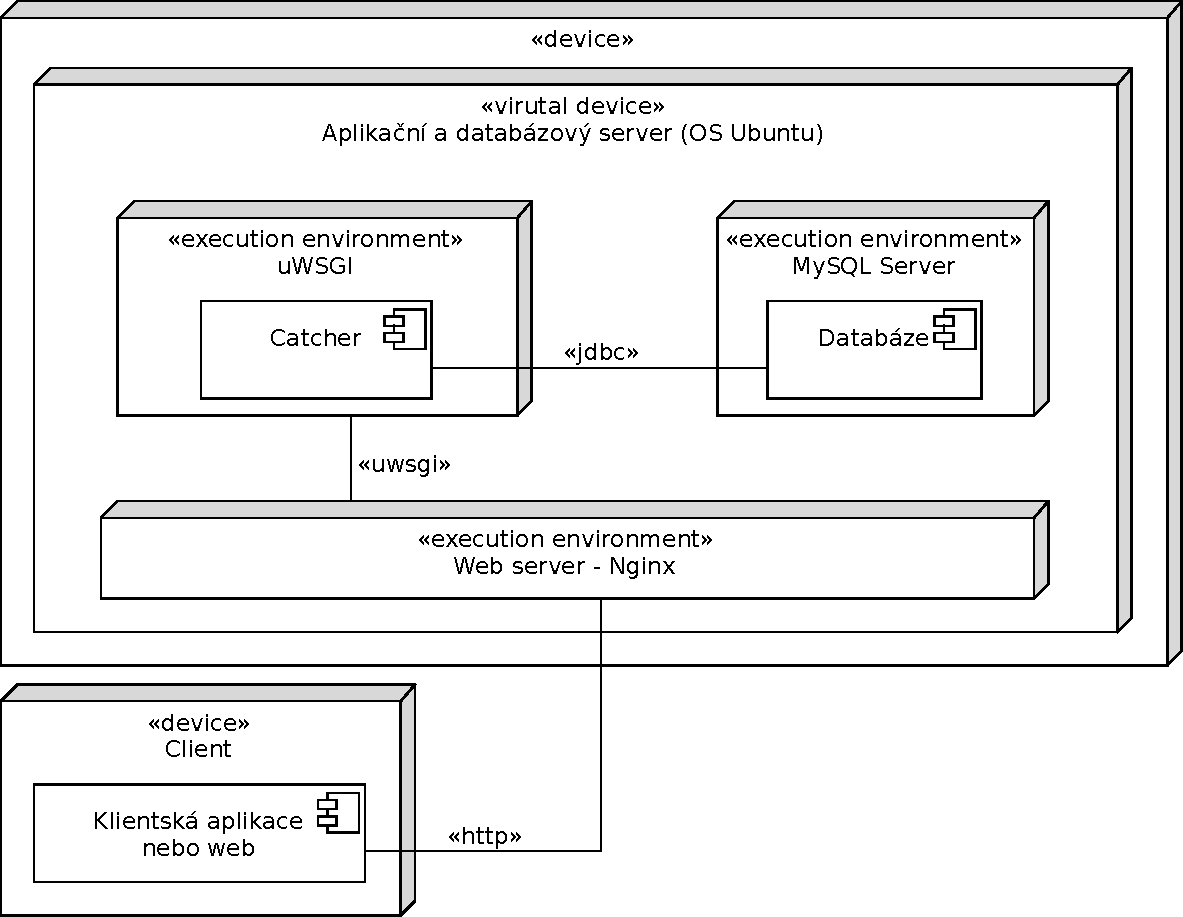
\includegraphics[width=130mm]{./images/diagram-nasazeni.pdf}
\caption{Diagram nasazení\label{overflow}}
\end{figure}

\section{uWSGI}

Aby bylo lépe pochopitelné zapojení uWSGI do celého procesu nasazení, popíšeme si jej trochu detailněji.

Projekt uWSGI je malý program, který se stará o management procesu aplikace.
Funguje jako prostředník mezi webovým serverem a aplikací,
se kterými komunikuje vlastním uwsgi protokolem, respektive standardním WSGI.
Detail komunikace je vidět na obrázku~\ref{fig:uwsgi}.

\begin{figure}[ht!]
\centering
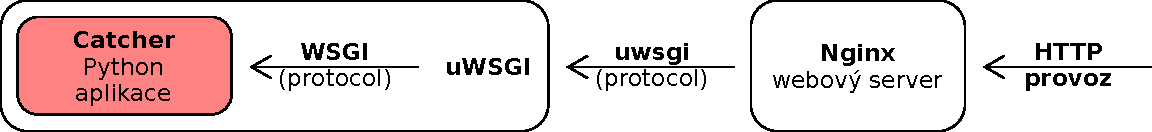
\includegraphics[width=135mm]{./images/uwsgi.pdf}
\caption{Komunikace mezi webovým serverem a aplikací v Pythonu; zdroj:~autor na základě~\cite{uwsgi}\label{overflow}}
\label{fig:uwsgi}
\end{figure}

\subsection*{uWSGI úloha}

Spuštění webové aplikace provadím následujícím příkazem. Proces poslouchá na~portu 8080, odkud přijímá zprávy od~webového serveru, a~po~celou dobu běží na~pozadí.

\begingroup
\fontsize{9.5pt}{11pt}\selectfont
\begin{verbatim}
$ uwsgi --socket localhost:8080 --wsgi-file ./restapi.py --callable api &
\end{verbatim}
\endgroup

\section{Konfigurace}

\subsection*{Konfigurační soubor}

Protože všechny moje zdrojové kódy byly zveřejněny v repozitáři na Git\-Hubu, nebylo by správné, aby obsahovaly jakákoliv hesla.
Pro tyto potřeby byl vytvořen konfigurační soubor, který mám zazálohovaný na vlastním cloudovém úložišti
a~pomocí programu wget~\cite{wget} si jej stahuji do~projektu vždy, když je změněn.
Tento konfigurační soubor obsahuje hesla k~produkční a~testovací databázi
nebo k~e-mailovému účtu, který používám pro~obnovu hesla uživatelů.

\subsection*{Databáze}

Pro přístup do databáze bylo potřeba vytvořit uživatele s~právem zapisovat, číst a mazat.
Tento účet se nadále autentizuje heslem, které je uložené v~konfiguračním souboru.
Příkazy pro vytvoření uživatele v SQL jsou následující:

\begingroup
\fontsize{9.5pt}{11pt}\selectfont
\begin{verbatim}
CREATE USER 'catcher-server'@'localhost' IDENTIFIED BY 'tajne_heslo';
GRANT SELECT, INSERT, UPDATE, DELETE
    ON catcher. * TO 'catcher-server'@'localhost';
\end{verbatim}
\endgroup

\subsection*{Nginx}

Protože disponuji pouze jednou veřejnou adresou na VPS, bylo potřeba webový server nakonfigurovat tak,
aby dokázal obsluhovat požadavky webové aplikace i požadavky
na zobrazení dokumentace. Konfigurace na serveru byla následující:

\begingroup
\fontsize{9.5pt}{11pt}\selectfont
\begin{verbatim}
upstream catcher_uwsgi {
    # adresa a port, na které přeposílám požadavky pro Catchera
    server localhost:8080;
}

server {
    # číslo portu na ipv4
    listen       80;
    # číslo portu na ipv6
    listen       [::]:80;
    # jméno serveru
    server_name  catcher.zlutazimnice.cz *.catcher.zlutazimnice.cz;
    charset      utf-8;
    index        index.html;
    
    # maximální velikost uploadu
    client_max_body_size 75M;

    # dokumentace na catcher.zlutazimnice.cz
    location / {
        # adresář s obsahem webu
        root   /var/www/catcher;
    }

    # webová aplikace na catcher.zlutazimnice.cz/api
    location /api {
        include     uwsgi_params;
        # upstream pro spojení s uwsgi
        uwsgi_pass  catcher_uwsgi;
    }
}
\end{verbatim}
\endgroup

Pro vývoj na svém počítači jsem použil trochu odlišnou konfiguraci, protože
jsem nemusel na jedné adrese provozovat dokumentaci i aplikaci.
V prvních fázích vývoje jsem dokonce ani Nginx používat nemusel, protože uWSGI umožňuje simulovat
chování webového serveru.
Pro produkční nasazení ale~není tento postup doporučen.

\section{Údržba}

Standardem pro větší aplikace by měl být monitorovací systém,
který sleduje zátěž jednotlivých komponent (webová aplikace, databáze, webový server atd.)
a~v~případě výpadku informuje administrátora SMS zprávou nebo e-mailem.
Pro potřeby Catchera jsem však využil daleko jednodušího řešení -- webové aplikace Uptime Robot~\cite{uptime_robot},
která v pravidelných intervalech \uv{oťukává} mnou definovavné adresy a~ověřuje jejich dostupnost.
Pro použití v~omezené míře je zdarma a~v~situaci, kdy je Catcher nedostupný, mě informuje e-mailem.


%by mělo stačit \uv{oťukávání} z testovacíh

%~\cite{uptime_robot}


%Pro potřeby Catchera by mělo stačit \uv{oťukávání} z testovacíh

%Až bude Catcher nasazen do ostrého provozu, pro jeho potřeby by měl stačit Cron\footnote{Jde o softwarového démona, který slouží
%k~automatickému spouštění periodicky se opakujících příkazů a procesů.},
%který by v~pravidelných intervalech \uv{oťukával} aplikaci a~stanovil, zda korektně běží.

Dále je nutné pro případ výpadku pravidelně zálohovat databázi. Místo manuálního zálohování programem
\texttt{mysqldump}~\cite{mysqldump}, lze použít Cron\footnote{Jde o softwarového démona, který slouží
k~automatickému spouštění periodicky se opakujících příkazů a procesů.}, který by pravidelně tento program spouštěl. 
V~případě výpadku by tak stačilo aplikaci opravit a~nahrát poslední zálohu.
Catcher aktuálně disponuje pouze manuálním zálohováním databáze.



% TODO: IDEA: Pouzit nasledujici:

%\section{Co by šlo udělat lépe}
%Během vývoje jsem se setkal se zajímavými nástroji, na které v tomto projektu nezbyla kapacita. Jejih použití by přineslo několik zlepšení, proto jsem se rozhodl je zde uvést:
%list:
%Virtualenv, Codevoc, Travis CI
%IDEA: Lze se zminit o testovani a prubezne integraci. Napriklad napsat, ze mame zajem v budoucnu pouzivat Codevoc (mozna spis testovani) nebo Travis CI.

\begin{conclusion}

% TODO: uvest, ze ta aplikace je sice naimplementovana, ale jeste ji neco malo chybi

  V práci jsem pro lepší pochopení uvedl čtenáře do problematiky, analyzoval již fungující i možná řešení
  a~provedl návrh backendu, ze kterého vzešlo řešení vytvořit webovou službu nezávislou na webové aplikaci.
  Službu se podařilo implementovat pomocí jazyka Python a úspěšně nasadit na virtuální privátní server.
  Důležitým výsledkem je také sepsání dokumentace a vytvoření automatizovaných testů pro~lepší odhalování chyb,
  jimiž mohu usnadnit práci nejen sobě, ale i všem dalším programátorům, kteří se budou na vývoji v budoucnu podílet. % Hlavním úspěchem je tak kompletní dokončení projektu.
  
  Teď, když je celá práce za mnou, mohu s odstupem prohlásit, že více času jsem se měl věnovat návrhové části.
  Systém měl být daleko více objektově orientovaný. Ve zdrojových kódech dochází k nelogickému umístění částí kódu,
  které se měly nacházet na vhodnějších místech, například v třídních metodách a ne ve funkcích apod.
  Kromě toho je určitě prostor pro zlepšení webové služby po stránce bezpečnosti, především použití protokolu HTTPS.
  
  Hlavním cílem práce bylo navrhnout a implementovat backend pro webovou aplikaci. I přesto, že moje původní představa
  týkající se malého rozsahu práce byla poměrně naivní, úspěšně jsem dokončil hlavní i~dílčí cíle. Webová aplikace kolegy Jaroslava Veselého
  úspěšně využívá moje řešení a na základě naší debaty máme další nápady, jak aplikaci rozšířit. Na základě analýzy jsme také zjistili,
  že podobná aplikace pro jednoduchou správu turnajů v Ultimate Frisbee zde chybí a úspěšným dokončením této práce jsme vyplnili díru na~trhu.  
\end{conclusion}

% TODO: Promyslet, jak presne odevzdavat citace.
%\bibliographystyle{csn690}
%\bibliographystyle{iso690}
%\bibliography{ref}

\begin{thebibliography}{1}

\bibitem{ultimate-time} BERNACCHI, Chris a Bryan WALSH. Don’t Let the IOC\
Ruin Ultimate Frisbee. TIME [online]. 2015 [cit. 2016-04-27].\
Dostupné z: http://time.com/3982671/dont-let-the-ioc-ruin-ultimate-frisbee/

\bibitem{cald-ultimate} Co je Ultimate? Česká Asociace Létjícího Disku [online].\
[cit. 2016-04-27]. Dostupné z: http://cald.cz/co-je-ultimate

\bibitem{usa-ultimate} What is Ultimate? USA Ultimate: About Ultimate [online].\
2015 [cit. 2016-04-27]. Dostupné z: http://www.usaultimate.org/about/

\bibitem{cald-uznani} KOTĚŠOVEC, Petr. ČALD získala oficiální uznání od Českého Olympijského Výboru.\
In: Česká Asociace Létjícího Disku [online]. 2015 [cit. 2016-04-27].\
Dostupné z: http://cald.cz/novinky/cald-ziskala-oficialni-uznani-od-ceskeho-olympijskeho-vyboru

\bibitem{cald-historie} Historie ultimate. Česká Asociace Létjícího Disku [online].\
[cit. 2016-04-27]. Dostupné z: http://cald.cz/historie-ultimate

\bibitem{cald-kalendar} Kalendař. Česká Asociace Létjícího Disku [online].\
[cit. 2016-04-27]. Dostupné z: http://cald.cz/kalendar

\bibitem{cald-catcher} VOSEČEK, Jiří, Ondřej BURKERT a Petr KOTĚŠOVEC.\
Mobilní aplikace pro skórování na turnajích.\
In: Česká Asociace Létjícího Disku [online]. 2013 [cit. 2016-04-29].\
Dostupné z: http://cald.cz/novinky/mobilni-aplikace-pro-skorovani-na-turnajich

\bibitem{catcher-play} Catcher. Google Play [online]. 2016 [cit. 2016-04-29].\
Dostupné z: https://play.google.com/store/apps/details?id=com.ulti.catcher\&hl=cs

\bibitem{http_metody} GOURLEY, David a Brian TOTTY. HTTP: the definitive guide.\
1st ed. Sebastopol, CA: O’Reilly, 2002, xviii, 635 p. ISBN 15-659-2509-2.

%GOURLEY, David a Brian TOTTY. HTTP: the definitive guide. 1st ed. Sebastopol, CA: O’Reilly, 2002, xviii, 635 p. ISBN 15-659-2509-2.

\bibitem{ultimate-organizer} Ultimate Organizer. SourceForge [online].\
2016 [cit. 2016-04-29]. Dostupné z: https://sourceforge.net/projects/ultiorganizer/

\bibitem{rest_vse} KOUDELKA, Jakub. Metodika návrhu REST API.\
Praha, 2013. Diplomová práce. Vysoká škola ekonomická v Praze. Vedoucí práce Lukáš Burkoň.

\bibitem{uri_wiki} URI scheme. In: Wikipedia: the free encyclopedia [online]. San Francisco (CA): Wikimedia\
Foundation, 2001- [cit. 2016-04-24]. Dostupné z: http://en.wikipedia.org/wiki/URI\_\
scheme

\bibitem{python-year} VAN ROSSUM, Guido. A Brief Timeline of Python.\
In: The History of Python [online]. 2009 [cit. 2016-04-26]. Dostupné z:\
http://python-history.blogspot.cz/2009/01/brief-timeline-of-python.html

\bibitem{python-companies} COCHRANE, Ken. Best Python Companies to Work For.\
In: DZone [online]. 2012 [cit. 2016-04-26]. Dostupné z:\
https://dzone.com/articles/best-python-companies-work

\bibitem{python-pypl} PYPL Index. PYPL PopularitY of Programming Language\
[online]. 2016 [cit. 2016-04-26]. Dostupné z: http://pypl.github.io/PYPL.html

\bibitem{falcon-benchmarks} Benchmarks. Falcon - The minimalist Python WSGI\
framework [online]. [cit. 2016-04-26]. Dostupné z: http://falconframework.org/

\bibitem{nginx-statistic} February 2016 Web Server Survey. Netcraft [online].\
2016 [cit. 2016-04-27]. Dostupné z: http://news.netcraft.com/archives/2016/02/22/february-2016-web-server-survey.html

\bibitem{nginx-changes} Changes. Nginx [online]. 2004 [cit. 2016-04-27].\
Dostupné z: http://nginx.org/en/CHANGES

\bibitem{fielding} FIELDING, Roy Thomas. Architectural styles and the design of network-based\
software architectures. Irvine, 2000. ISBN 0-599-87118-0. Disertační.\
University of California, Irvine. Vedoucí práce Richard Taylor.

\bibitem{uwsgi} PRAUS, Petr. Produkční nasazení Django aplikací na Cherokee pomocí WSGI.\
In: Zdroják.cz [online]. 2010 [cit. 2016-04-29]. Dostupné z:\
https://www.zdrojak.cz/clanky/produkcni-nasazeni-django-aplikaci-na-cherokee-pomoci-wsgi

\end{thebibliography}

\appendix
% 
\chapter{Seznam použitých zkratek}
% \printglossaries
\begin{description}
	\item[ČALD] Česká asociace létajícího disku
	\item[SOTG] Spirit of the Game
	\item[URI] Uniform Resource Identifier
	\item[URL] Uniform Resource Locator
	\item[GUI] Graphical user interface
	\item[API] Application Programming Interface
	\item[SOAP] Simple Object Access Protocol
	\item[REST] Representational State Transfer
	\item[CRUD] Create, read, update and delete
	\item[XML] Extensible markup language
	\item[JSON] JavaScript Object Notation
	\item[UML] Unified Modeling Language
	\item[ORM] Object-relational mapping
	\item[SQL] Structured Query Language
	\item[HTML] HyperText Markup Language
	\item[CSS] Cascading Style Sheets
	\item[HTTP] Hypertext Transfer Protocol
	\item[HTTPS] Hypertext Transfer Protocol Secure

\end{description}

\chapter{Datový model}
  \label{appendix:data_model}
  \begin{figure}[ht!]
    \centering
    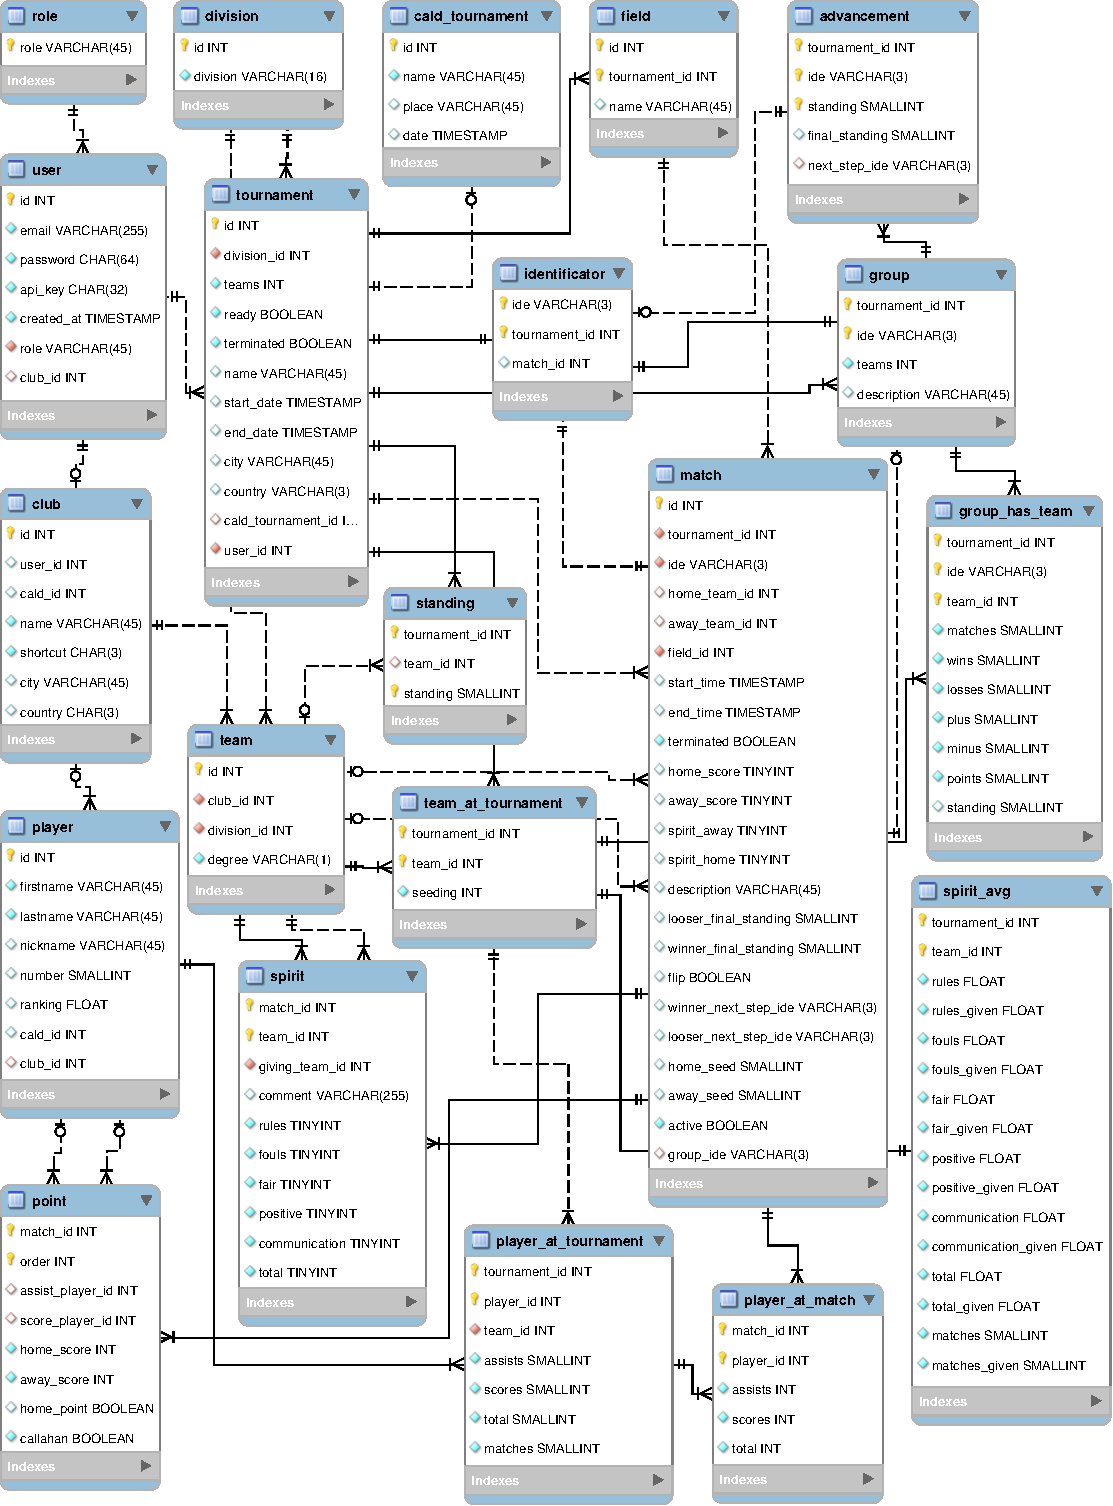
\includegraphics[width=95mm]{./images/datovy-model.pdf}
    \caption{Datový model.\label{overflow}}
    \label{fig:domain_model}
  \end{figure}

\chapter{Obsah přiloženého CD}

%upravte podle skutecnosti

\begin{figure}
	\dirtree{%
		.1 readme.txt\DTcomment{stručný popis obsahu CD}.
		.1 exe\DTcomment{adresář se spustitelnou formou implementace}.
		.1 src.
		.2 impl\DTcomment{zdrojové kódy implementace}.
		.2 thesis\DTcomment{zdrojová forma práce ve formátu \LaTeX{}}.
		.1 text\DTcomment{text práce}.
		.2 thesis.pdf\DTcomment{text práce ve formátu PDF}.
		.2 thesis.ps\DTcomment{text práce ve formátu PS}.
	}
\end{figure}

\end{document}

% KDYBYCH NEKDY CHTEL POUZIT:

%\begin{description}
%  \item[Snadná rozšířitelnost] \hfill \\
%  Už nyní evidujeme změny, o které je zájem, ale nejsou předmětem této práce.
%  I proto je nutné projekt dokončit tak, aby byl v budoucnu snadno rozšiřitelný nebo
%  modifikovatelný.
%\end{description}

% TODO: tahle tabulka ma sirsi radky
% \renewcommand{\arraystretch}{1.5}
% 
% \begin{table}[ht!]
%  \begin{tabular}{ |l|l|l|l|  }
% \hline
% Zdroj & URL & Dostupné HTTP metody & popis \\
% \hline
% x & /login & x &  \\
% \hline
% Aland Islands & AX & ALA & \\
% Albania &AL & ALB & \\
% Algeria    &DZ & DZA & \\
% American Samoa & AS & ASM & \\
% Andorra & AD & AND &  \\
% Angola & AO & AGO &\\
% \hline
% \end{tabular}
% \caption{...}
% \end{table}

\iffalse
\fi